% !TeX root = ./main.tex

\documentclass[12pt, a4paper,oneside, toc=indentunnumbered,toc=chapterentrywithdots,german]{scrreprt}

\usepackage{caption,        % better captions
            courier,        % add courier for monospaced font when using \texttt
            listings,       % code snippets
            calc,           % calculate sizes e.g. \widthof{}
            enumitem,       % customize list environments 
            graphicx,       % including images
            tabularx,       % better tablesi
            booktabs,       % prettier tables
            pdfpages,       % inlcude pdf documents
            xurl,           % break urls at any alphanumeric character
            nameref,        % reference to paragraphs by name
            amsmath,
            graphicx
          }

\usepackage[english,main=ngerman]{babel} % german and english language package
\usepackage[utf8]{inputenc}         
\usepackage[T1]{fontenc}    % encoding, for german
\usepackage{lmodern}        % better representation 
\usepackage[left=25mm,right=25mm,top=25mm,bottom=25mm]{geometry}  % change document size
\usepackage[hidelinks]{hyperref} % remove colored ref-links 
\usepackage[ngerman,noabbrev]{cleveref} % references with german text
\usepackage[style=ieee, backend=biber]{biblatex}
\usepackage{csquotes} % enquote text, loading csquotes before inputenc to remove warnings

% \DeclareLanguageMapping{ngerman}{ngerman-apa} % set languagemapping to use apa style with biber
\bibliography{src/bibliography}


\renewcommand{\arraystretch}{1.2} % more space between rows in tables, maybe change to 1.3

\linespread{1.25}
%\onehalfspacing % set linespacing to 1.5

\renewcommand{\familydefault}{\sfdefault}

\lstset{literate=%
    {Ö}{{\"O}}1
    {Ä}{{\"A}}1
    {Ü}{{\"U}}1
    {ß}{{\ss}}1
    {ü}{{\"u}}1
    {ä}{{\"a}}1
    {ö}{{\"o}}1
    {~}{{\textasciitilde}}1,
    escapeinside={(@*}{*@)},
    captionpos=b,
    breakatwhitespace=true,
    breaklines=true,
    postbreak=\mbox{\textcolor{red}{$\hookrightarrow$}\space},
}

\renewcommand\lstlistingname{Listung} % rename captions for listings
\renewcommand\lstlistlistingname{Listungsverzeichnis} % rename header for list of listings

\crefname{listing}{Listung}{Listungen}
\Crefname{listing}{Listung}{Listungen}

\begin{document}
% !TeX root = ../paper.tex

\begin{titlepage}

\includegraphics[height=2.5cm]{images/dhbw.png}
\begin{center}
    \vspace*{\baselineskip}{\LARGE \textbf {Machbarkeitsstudie von 3D-Rekonstruktion mit OpenCV}\\
    \vspace*{2\baselineskip}{\Large \textbf{Studienarbeit}}\\
    \vspace*{2\baselineskip}{\large \textbf{des Studiengangs Angewandte Informatik}}\\
    \vspace*{.25\baselineskip}{\large \textbf{an der Dualen Hochschule Baden-Württemberg Mannheim}}\\
    \vspace*{2\baselineskip}{\large \textbf{von}}\\
    \vspace*{.25\baselineskip}{\Large{\textbf{Jan Maier, Sebastian Schmitt}}}\\
    \vspace*{2\baselineskip}{\large \textbf{Abgabedatum: 29.04.2020}}}
\end{center}
\vfill
\begin{tabularx}{\textwidth}{Xl}
    Matrikelnummer, Kurs & , TINF17AIBC \\
    Matrikelnummer, Kurs & 8608772, TINF17AIBC \\
    Betreuer der Hochschule & Prof. Dr. Eckhard Kruse \\
\end{tabularx}
\end{titlepage}


% set the page numbering for the frontmatter to roman
\pagenumbering{Roman}

% !TeX root = ../main.tex

\addchap{Abstract}
\paragraph{Deutsch}\mbox{}\\
Diese Arbeit behandelt das Thema Structure from Motion, also das Rekonstruieren einer Struktur aus mehreren Bildern.
Im Rahmen dieser Arbeit wird ein Konzept einer Pipeline zum Rekonstruieren eines Objekt aus mehreren Bildern vorgestellt und implementiert.
Für die Implementierung wird C++, so wie die Bibliothek OpenCV verwendet.
Ziel des Projekts ist es, die Rekonstruktionspipeline so zu implementieren, dass keine Unkosten durch patentierte Algorithmen oder kostenpflichtiger Software und Tools entstehen.
Die Implementation wird beschrieben und theoretische Grundlagen werden im Voraus erläutert. 
Das Ergebnis des Projekts wird zum Schluss an Hand von vier Testfällen evaluiert.
Die Testfälle zeigen verscheiden Objekte mit unterschiedlichen Eigenschaften.
Die Ergebnisse der Testfälle werden zusammengefasst und es werden mögliche Fehlerursachen bei der Rekonstruktion näher erläutert.
Zum Schluss werden mögliche weitere Vorgehensweisen und Ansätze zur Behebung der Fehler beschrieben. 

\paragraph{English}\mbox{}\\
 

% \addcontentsline{toc}{chapter}{\protect\numberline{}\tab}
\tableofcontents

% \newpage
% \addcontentsline{toc}{chapter}{\protect\numberline{}Abkürzungsverzeichnis}
\addchap*{Abkürzungsverzeichniss}

\begin{table}[h!]
    % \caption*{Abkürzungsverzeichnis}
    \begin{tabularx}{\textwidth}{l X}
        \toprule 
        Abkürzung & Bedeutung \\
        \midrule
        lorem & ipsum \\
        ipsum & lorem \\
        \bottomrule 
    \end{tabularx}
\end{table}


\newpage
\phantomsection
\addcontentsline{toc}{chapter}{\protect\numberline{}\listfigurename}
\listoffigures

\newpage
\phantomsection
\addcontentsline{toc}{chapter}{\protect\numberline{}\listtablename} 
\listoftables

\newpage
\phantomsection
\addcontentsline{toc}{chapter}{\protect\numberline{}\lstlistlistingname}
\lstlistoflistings


% mainmatter
\newpage
\pagenumbering{arabic}
% !TeX root = ../main.tex

\chapter{Motivation}
Echte Objekte mit virtuellen 3D Objekten abzubilden ist nicht einfach. Je nach Komplexität des Objekts sind Designer mehrere Tagen oder gar Wochen beschäftigt.
Dieser Vorgang kann mittels Photogrammetrie teilweise automatisiert und vereinfacht werden.
Photogrammetrie wird hauptsächlich zur Herstellung von topographischen Karten angewendet\cite{kraus_2004}.
Darüber hinaus gibt es aber auch besondere Anwendungsfälle.
Beispielsweise nutzen die Entwickler des Videospiels \emph{Chernobylite} Techniken der Photogrammetry um Chernobyl so genau wie möglich in ihrem Spiel nachzubilden\footnote{siehe dazu https://youtu.be/D3KM\_Rd1ReE}.
% !TeX root = ../main.tex

\chapter{Ziele und Anforderungen}\label{sec:goals}
Ziel der Arbeit ist es mit einfachen Mitteln eine Anwendung zur 3D-Rekonstruktion von Bildern zu entwickeln und die Machbarkeit davon zu bewerten.
Die Anwendung soll dabei aus einer Menge versetzter Bilder eines Objekts 3D Punkte des Objekts rekonstruieren und exportieren.
Dieses Vorgehen wird als Structure from Motion\footnote{Siehe dazu \autoref{sec:sfm} \nameref{sec:sfm}} bezeichnet.

Im folgenden Sind einzelne Ziele gesondert aufgeführt und erläutert.

\section{Ziele}
\begin{enumerate}
\item \label{goal:nocost} Für die Entwicklung und Nutzung der Software sollen keine Kosten entstehen
\item Bei der Entwicklung wird nach Möglichkeit auf offene Bibliotheken zurückgegriffen und möglichst wenig selbst implementiert
\end{enumerate}


\section{Anforderungen}
\begin{enumerate}
\item Es werden nur frei verfüg- und verwendbare Algorithmen verwendet um Ziel \autoref{goal:nocost} gerecht zu werden
\item  Die exportierten 3D Punkte lassen sich mit Blender\footnote{https://www.blender.org/} visualisieren
\item Die entwickelte Software soll unter aktuellen Versionen des Windows Betriebssystems lauffähig sein
\end{enumerate}

% !TeX root = ../../main.tex

\chapter{Stand der Technik}

\section{Was ist Photogrammetrie?}\label{sec:what-is-photogrammetry}
Mit Photogrammetrie bezeichnet man Techniken, mit denen man Informationen wie Position, Orientierung, Form und Größe eines Objekts aus Bildern rekonstruieren kann.
Dabei unterscheidet man ob es sich bei den Bildern um photochemische (konventionelle Photographie), photoelektrische (digitale Photographie) oder um Laserscanner-Aufnahmen\footnote{Bilder welche zusätzlich Entfernungsinformationen zu jedem Bildelement enthalten} handelt.
Je nach Art der Weiterverarbeitung sowie Aufnahme der Bilder wird der Begriff der Photogrammetrie weiter differenziert.
Bei Weiterverarbeitung von photochemischen Bildern mittels optisch-mechanischer Geräte spricht man von \textbf{analoger Photogrammetrie}.
Bei Weiterverarbeitung von photochemischen Bildern mittels Computer spricht man von \textbf{analytischer Photogrammetrie}.
Bei Weiterverarbeitung von photoelektrischen Bildern mittels Computer, ein voll digitaler Prozess, spricht man von \textbf{digitaler Photogrammetrie}.
Die Ergebnisse einer Auswertung mittels Photogrammetrie können sein: \cite[Kapitel 1.1]{kraus_2004}
\begin{itemize}
\item \textbf{Maßzahlen}, Koordinaten einzelner Objektpunkte in einem dreidimensionalen Koordinatensystem
\item \textbf{Zeichnungen}, Karten und Pläne im Grundriss mit Höhenlinien
\item \textbf{geometrische Modelle}
\item \textbf{Bilder}, entzerrte Fotos, Luftbildkarten
\end{itemize}

In dieser Arbeit werden Techniken der digitalen Photogrammetrie verwendet mit dem Ziel Maßzahlen als Ergebnis zu erhalten.

\section{Definitionen \& Begriffe}

\subsection{Structure from Motion}\label{sec:sfm}
Unter Structure from Motion, kurz SfM, versteht man eine Methode zur Rekonstruktion von 3D Punkten.
Im Gegensatz zur herkömmlichen Photogrammetrie, bei der zuvor bekannte 3D Punkte benötigt werden, wird bei SfM die Geometrie der Szene, Kamerapositionen und Orientierung berechnet.
Informationen wie Postionen der Kamera oder Kameraabstand sind vorab nicht  bekannt.
Wie in \autoref{fig:theory-sfm-images} zu sehen arbeitet man bei SfM nicht wie bei der normalen Photogrammetrie mit einem Stereo-Bildpaar sondern mit einer Menge leicht verschobener, sich überlappender Bilder.
Dieses Vorgehen bietet sich also vor allem für Mengen von Bildern an, welche sich zu einem hohen Grad überlappen aber gleichzeitig eine dreidimensionale Struktur zeigen.
~\cite[Kapitel 1.2]{westoby_2012}

\begin{figure}
    \centering
    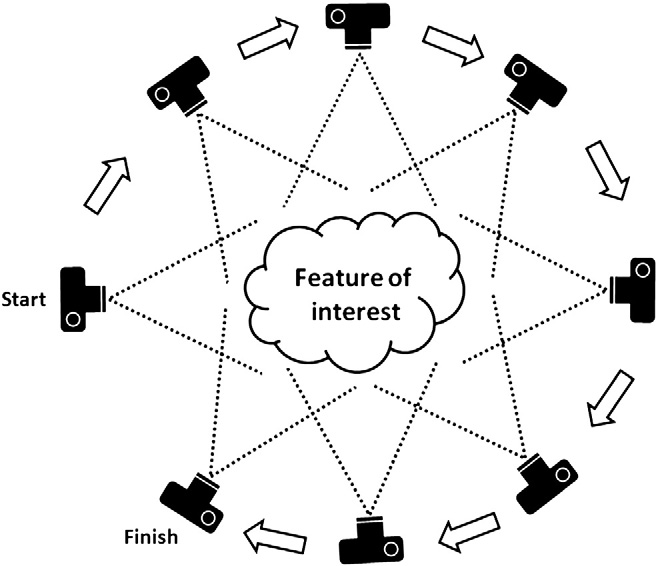
\includegraphics[width=\textwidth]{src/img/westoby_2012_fig1_sfm_images.jpg}
    \caption{Für Structure from Motion werden statt einem Stereo-Paar mehrere, sich überlappende Bilder benötigt~\cite[Fig. 1]{westoby_2012}}
    \label{fig:theory-sfm-images}
\end{figure}

Dieses Vorgehen macht sich die Parallaxe zu nutze\cite[stockmann_2001].
Mit Parallaxe bezeichnet man die scheinbare Änderung der Position eines Objektes, wenn der Beobachter seine eigene Position ändert.
Definiert ist diese als der Winkel zwischen zwei Geraden, welche von verschiedenen Standorten auf denselben Punkt (ein Objekt) gerichtet sind (Siehe dazu \autoref{fig:theory-sfm-parallax}) \cite{stockmann_2001}.
\footnote{Als anschauliches Beispiel kann man bei ausgestrecktem Arm einen Daumen heben und diesen abwechselnd mit dem linken und dem rechten Auge betrachten.}

\begin{figure}
    \centering
    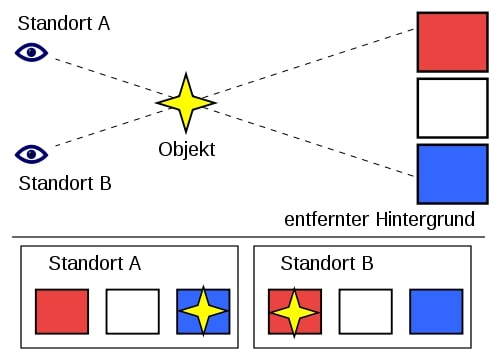
\includegraphics[width=\textwidth]{src/img/500px-Parallax_Example_de.jpg}
    \caption{Beispiel einer Parallaxe~\cite{wiki:parallax_example_de}}
    \label{fig:theory-sfm-parallax}
\end{figure}

Um die Kameraposition sowie die Geometrie der Szene simultan zu rekonstruieren werden automatisch Feature in den Bildern identifiziert.
Diese Feature werden dann über mehrere Bilder verfolgt, was eine erste Annahme zu den Kamerapositionen sowie den Objektkoordinaten erlaubt.
Sie können iterativ mittels nicht-linearer least-squares minimisation verfeinert werden. ~\cite[Kapitel 1.3]{westoby_2012}

\subsection{Lochkamera-Modell}\label{sec:pinhole-camera-model}
Das Lochkamera-Modell ist das einfachste Kameramodell und wird im Folgenden dazu verwendet relevante Begriffe und die Geometrie zu erklären.
Bei diesem Modell wird die zentrale Projektion von Punkten im Raum auf eine Ebene betrachtet.
Das Zentrum der Projektion definiert den Ursprungs eines euklidischen Koordinatensystems.
Dieser wird auch \emph{Kamerazentrum} genannt und als Punkt $C$ referenziert.
Die Bildebene liegt parallel zu der XY-Ebene auf der Z-Achse.
Der Abstand zum Ursprung wird durch die Brennweite $f$ der Kamera definiert.
Der Schnittpunkt $p$ der Bildebene und der Z-Achse wird als Hauptpunkt (engl. principal point) bezeichnet und definiert innerhalb der Bildebene den Ursprung eines zweidimensionalen Koordinatensystems.
Häufig ist es aber der Fall, dass der Hauptpunkt und der Ursprung voneinander abweichen.
Daher wird der Ursprung auch mit den Koordinaten $(p_x, p_y)^T$ angegeben.
Mit diesen Informationen kann nach~\cite[Gleichung 6.2]{hartley_2003} die Abbildung eines Punkts im Raum auf die Bildebene in homogenen Koordinaten durch eine Matrixmultiplikation ausgedrückt werden:
\begin{equation}
\label{eqn:theory-projection}
\begin{pmatrix}
    X \\ Y \\ Z \\ 1
\end{pmatrix}
\mapsto
\begin{pmatrix}
    fX+Zp_x \\ fY+Zp_y \\ Z
\end{pmatrix}
=
\begin{bmatrix}
    f &   & p_x & 0 \\
      & f & p_y & 0 \\
      &   & 1   & 0
\end{bmatrix}
\begin{pmatrix}
    X \\ Y \\ Z \\ 1
\end{pmatrix}
\end{equation}
Diese Gleichung lässt sich mit der Notation $X$ für einen homogenen 4-Vektor, $x$ für einen homogenen 3 Vektor als $x = PX$ schreiben.
Dabei ist $P$ die homogene $3\times 4$ \emph{Kamera-Projektionsmatrix} (auch \emph{Kamermatrix} oder \emph{Projektionsmatrix} genannt).
Mit der Definition der \emph{Kamera-Kalibrierungsmatrix} (auch \emph{Kalibrierungsmatrix}) K
\[
    K=
    \begin{bmatrix}
    f &   & p_x & 0 \\
      & f & p_y & 0 \\
      &   & 1   & 0
    \end{bmatrix}
\]
kann die~\autoref{eqn:theory-projection} auch zu $x=K[I | 0] X$ vereinfacht werden~\cite[vgl. Gleichung 6.5]{hartley_2003}. 


\begin{figure}
    \centering
    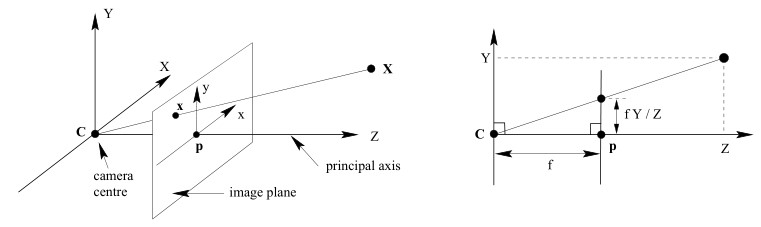
\includegraphics[width=\textwidth]{src/img/hartley_2003_lochkamera.jpg}
    \caption{Darstellung des Lochkamera-Modells~\cite[Fig. 6.1]{hartley_2003}}
    \label{fig:theory-pinhole-camera}
\end{figure}


Für gewöhnlich werden Punkte in einem Raum in einem anderem Koordinatensystem ausgedrückt.
Die Beziehung zwischen beiden Koordinatensystemen wird durch die $3\times 3$ Rotationsmatrix $R$ und dem Translationsvektor $t$ beschrieben. 
Die Kamera-Projektionsmatrix kann somit auch als $P=K[R|t]$ geschrieben werden~\cite[Kapitel 6.1,S. 156, Gleichung 6.7]{hartley_2003}.


\subsection{Fundamental Matrix}\label{sec:fundamental-mat}
Die Fundamental Matrix ist eine algebraische Darstellung der Epipolargeometrie zwischen zwei Sichten.
Ziel dieser Geometrie ist die Suche von korrespondierenden Punkten in zwei Sichten.

Man nehme an, dass der Raumpunkt $X$, die Bildpunkte $x$ und $x'$, und die Kamerazentren $C$ und $C'$ in einer Ebene, genannt $\pi$, liegen (siehe Abb.~\ref{fig:theory-fundamental-matrix}).
Man erkennt, dass sich die Linien von den Kamerazentren durch $x$ bzw. $x'$ in $X$ schneiden und ebenfalls in der Ebene liegen.
Mit dieser Eigenschaft kann man die Suche von korrespondierenden Bildpunkten vereinfachen.
Nimmt man an, dass man nur den Bildpunkt $x$ kennt, dann kann man mit Hilfe der Ebene $\pi$ die Position von $x'$ einschränken.
Denn $x'$ muss sich auf der Schnittlinie der eben beschriebenen Ebene und der Bildebene der zweiten Sicht befinden. 
Diese Schnittlinie wird \emph{Epipolarlinie} genannt.
Die Punkte $e$ und $e'$ sind die Schnittpunkte des Vektors $\overline{CC'}$ mit den Bildebenen und werden Epipole genannt.
Die Ebene $\pi$ wird zusätzlich Epipolarebene genannt~\cite[Kapitel 9,1]{hartley_2003}.

% S.240 / 241 multiple view geometry
Die Fundamental Matrix wird in~\cite[Kapitel 9.2]{hartley_2003} definiert als die $3\times 3$ Matrix, die für alle korrespondierenden Punkte $x \leftrightarrow x'$ 
\[ x'^TFx=0\] 
erfüllen.
Geometrisch betrachtet ist die Matrix F eine Abbildung der Punkte in einem Bild auf ihre Epipolarlinien im zweiten Bild.

\begin{figure}[h!]
    \centering
    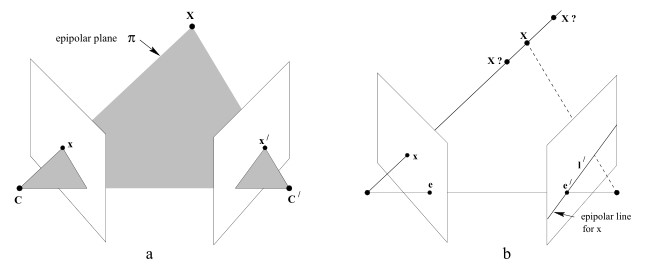
\includegraphics[width=\textwidth]{src/img/hartley_2003_fundamental_matrix.jpg}
    \caption{Veranschaulichung der Epipolargeometrie~\cite[Fig. 9.1]{hartley_2003}}
    \label{fig:theory-fundamental-matrix}
\end{figure}

\subsection{Essentielle Matrix}\label{sec:essential-mat}
Die essentielle Matrix ist eine Spezialisierung der Fundamentalmatrix mit normalisierten Bildkoordinaten.
Sie wird durch die Gleichung $\hat{x}'E\hat{x}$ definiert, wobei $\hat{x}$ ein Punkt in normalisierten Bildkoordinaten darstellt.
Mit Hilfe der Kalibrierungsmatrizen $K$ und $K'$ von zwei Bildern, kann die Beziehung $E=K'^TFK$ zur Fundamentalmatrix hergeleitet werden~\cite[Kapitel 9.6]{hartley_2003}.

Es ist möglich durch eine Singulärwertzerlegung der essentiellen Matrix die Kameramatrix zu bestimmen.
Dabei wird für die erste Kameramatrix $P=[I|0]$ angenommen. 
Für die zweite Kameramatrix gibt es vier Möglichkeiten, die sich aus den zwei möglichen Rotationsmatrizen $R$ und den zwei möglichen Vorzeichen für den Translationsvektor $t$ ergeben.
Geometrisch betrachtet kann jedoch nur einer der Kombinationen stimmen.
Wie in Abb.~\ref{fig:theory-essential-matrix-geometry} zusehen ist, gibt es nur einen Fall, bei dem ein Punkt im Raum vor beiden Bildebenen liegt.
Mit dieser Überprüfung kann die zweite Kameramatrix $P'=[R|t]$ bestimmt werden.
Hier muss beachtet werden, dass $t$ ein Einheitsvektor und nur maßstabsgetreu ist~\cite[Kapitel 9.6.3]{hartley_2003}.


\begin{figure}[h!]
    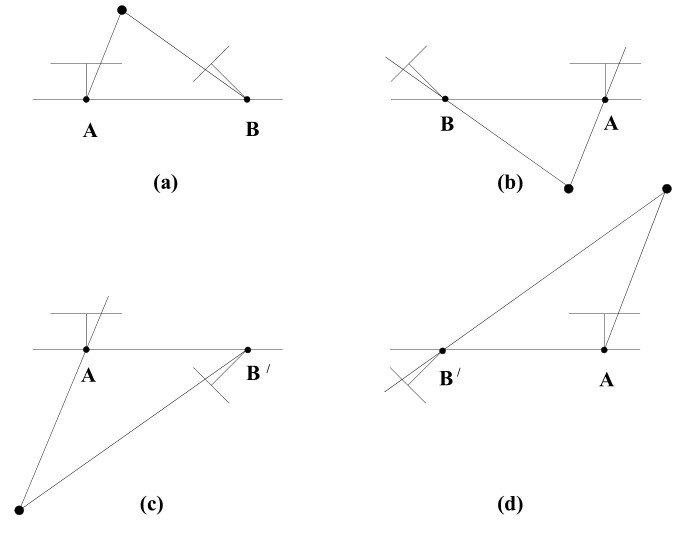
\includegraphics[width=\textwidth]{src/img/hartley_2003_e_geometry.jpg}
    \caption{Die geometrische Darstellung der vier möglichen Lösungen für $E$. Nur in (a) liegt der markierte Punkt vor beiden Kameraebenen~\cite[Fig. 9.12]{hartley_2003}}.
    \label{fig:theory-essential-matrix-geometry}
\end{figure}

\section{Kamerakalibrierung}\label{sec:theory-calibration}
Die Kamerakalibrierung ist ein Prozess zum Bestimmen der kamera-spezifischen Parametern der Kameramatrix und den Verzerrungsparametern. 
In \cref{sec:pinhole-camera-model} wird die Kameramatrix erklärt.
Die Verzerrungsparameter werden genutzt, um die Verzerrung auszugleichen, die durch der Kameralinse entsteht.
Hierbei wird zwischen zwei Arten der Verzerrung unterschieden: radiale und tangentiale Verzerrung.
Radiale Verzerrung entsteht durch die runde Form der Linse, wodurch die Pixel am Bildrand verzerrt werden.
Diese Verzerrung kann bei manchen Linsen zunehmen, je weiter ein Strahl entfernt vom Zentrum auf die Linse trifft. 
Diese Art der Verzerrung kann mathematisch als Taylorreihe um $r = 0$ und dem Termen $k_1, k_2$ und $k_3$ beschrieben werden.
Ein Punkt $(x, y)$ kann somit als $(x_{\text{corrected}},y_{\text{corrected}})$ ohne Verzerrung ausgedrückt werden, wobei gilt:
\[x_\text{corrected} = x \cdot (1 + k_1r^2 + k_2r^4 + k_3r^6)\]
\[y_\text{corrected} = y \cdot (1 + k_1r^2 + k_2r^4 + k_3r^6)\]
Tangentiale Verzerrung entsteht durch Herstellungsfehler, wodurch die Linse nicht genau parallel zur Abbildungsebene liegt.  
Sie wird durch die Parameter $p_1$ und $p_2$ beschrieben, wodurch ein Punkt $(x,y)$ durch $(x_{\text{corrected}},y_{\text{corrected}})$ ohne Verzerrung dargestellt wird. 
Dabei gilt:
\[x_\text{corrected} = x + (2p_1xy + p_2(r^2 + 2x^2))\]
\[y_\text{corrected} = y + (p_1(r^2 + 2y^2) + 2p_xy)\]
\cite{kaehler_2016}

Eine Kamera kann mit verschieden Methoden kalibriert werden.
Häufig werden bei den Methoden Referenzraster eingesetzt, wie z.B.\ ein Schachbrettmuster.
Das Referenzraster kann hierbei 2D oder auch 3D sein wie in den \cref{fig:2d_grid,fig:3d_grid} zu sehen ist.
Eine weitere Methode ist die Auto-Kalibrierung, bei der kein Kalibrierungsobjekt genutzt wird.
Dabei werden die Kameraeigenschaften aus unkalibrierten Bildern gewonnen, in dem Restriktionen auf die Kameraparameter oder auf die abgebildete Szene gelegt werden.
Die Auto-Kalibrierung wird häufig bei der 3D Modellierung eingesetzt~\cite{remondino_2005}.

\begin{figure}[h]
    \centering
    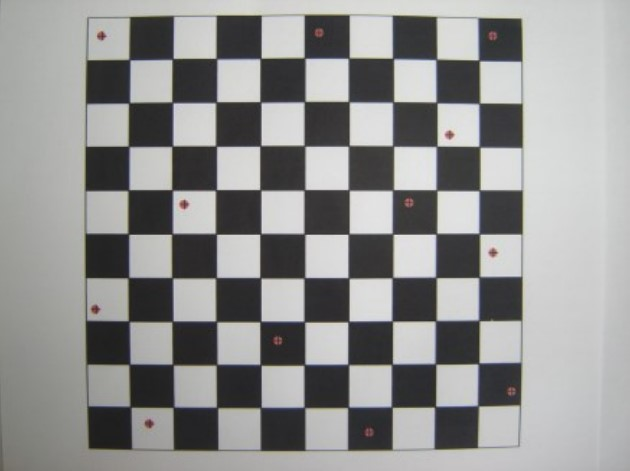
\includegraphics[width=\textwidth]{src/img/mendonca_2013_2d_grid.jpg}
    \caption{2D Referenzraster mit Schachbrettmuster für die Kamerakalibrierung (aus~\cite[Fig. 2]{mendonca_2013})}
    \label{fig:2d_grid}
\end{figure}



\begin{figure}[h]
    \centering
    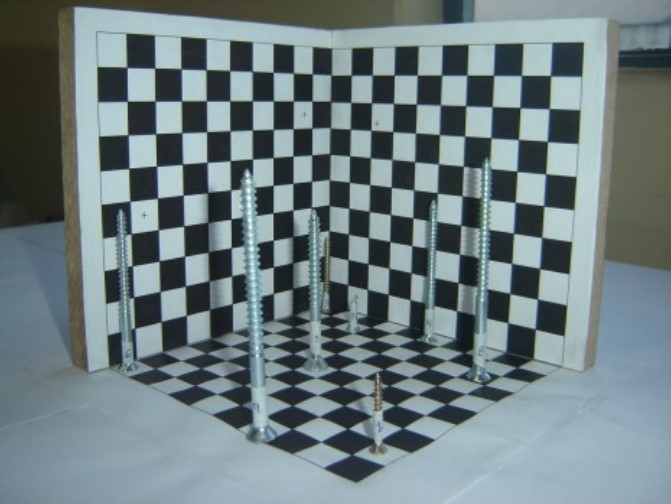
\includegraphics[width=\textwidth]{src/img/mendonca_2013_3d_grid.jpg}
    \caption{3D Referenzraster mit Schachbrettmuster für die Kamerakalibrierung (aus~\cite[Fig. 4]{mendonca_2013})}
    \label{fig:3d_grid}
\end{figure}

\section{Feature Matching}\label{sec:theory-feature-matching}
In vielen Computer Vision Anwendungen ist das Erkennen, Beschreiben und Finden von Übereinstimmungen von Features ein wichtiger Bestandteil~\cite{hassaballah_2016}.
Unter Anderem werden bei Methoden der 3D Rekonstruktion, wie SfM, korrespondierende Bildpunkte in verschiedenen Bildern benötigt, um eine abgebildete Szene rekonstruieren zu können.

In~\cite{hassaballah_2016} wird \emph{Feature Matching} als das Bilden von Korrespondenzen zwischen zwei Bildern der gleichen Szene bzw.\ des gleichen Objekts beschrieben.
Dazu werden Keypoints bzw.\ Features in den einzelnen Bildern erkannt und durch Deskriptoren beschrieben.
In~\cite[Kapitel 16]{kaehler_2016} werden Keypoints bzw.\ Features als \enquote{a small portion of an image that, for one reason or another, is unusually distinctive, and which we believe we might be
able to locate in another related image} beschrieben.
Im gleichen Buch werden die Deskriptoren beschrieben als \enquote{some mathematical construction, typically (but not always) a vector of floating-point values, which somehow describes an individual keypoint, and which can be used to determine whether---in some context---two keypoints are ``the same.''}
Mit Hilfe der Deskriptoren kann ein Distanzmaß definiert werden, um ihre Ähnlichkeit zu einander zu testen.

Algorithmen, die Features aus Bildern extrahieren, werden \emph{Feature Detector} genannt, während Algorithmen zum bilden der Deskriptoren \emph{Feature Descriptor} genannt werden~\cite{hassaballah_2016}.
In~\cite{hassaballah_2016} werden die folgenden Eigenschaft beschrieben, die wichtig für Feature Descriptors sind:
\begin{itemize}
    \item Robustheit: die Features sollten in der selben Position erkannt werden, unabhängig von der Skalierung, Rotation, Verschiebung etc.
    \item Wiederholbarkeit: Die selben Features der selben Szene bzw.\ Objekts sollen auch variierenden Konditionen wiedererkannt werden.
    \item Genauigkeit: Features sollen möglichst genaue Bildkoordinaten haben.
    \item Allgemeinheit: der Algorithmus sollte Features erkennen, die in verschiedenen Applikationen verwendet werden können.
    \item Effektivität: der Algorithmus soll möglichst schnell sein, um Echtzeit-Applikationen zu unterstützen. 
    \item Quantität: es sollen alle oder möglichst viele Features in einem Bild gefunden werden.
\end{itemize}
Wie wichtig die Eigenschaften im Vergleich zu einander sind, hängt von dem Anwendungsfall ab.




% !TeX root = ../../main.tex

\chapter{Konzept}
In diesem Abschnitt wird kurz unser Konzept für die Umsetzung von Sfm erläutert. 
Insbesondere wird dabei erläutert, was in den einzelnen Schritten durchgeführt wird, und warum diese Schritte notwendig sind.
Details zur Implementierung werden in Kapitel~\ref{sec:implementation} beschrieben.

Das Konzept ist eine Kommandozeilen-Applikation, welche eine Pipeline mit Prozessen zur Rekonstruktion von Bildpunkten bereitstellt.
Die Pipeline ist in Abb.~\ref{fig:concept-pipeline} dargestellt.
Parameter, die für die einzelnen Prozesse benötigt werden, werden als Kommandozeilen-Argumente übergeben.
Der erste Prozess \emph{Kalibrierung} bestimmt die Parameter der Kamera, mit der die Bilder zur Rekonstruktion aufgenommen wurden.
Dieser Schritt ist nötig, da bei der Rekonstruktion die Kalibrierungsmatrix K benötigt wird.
Diese Matrix enthält Informationen über die Brennweite der Kamera und der Position des Hauptpunkts im Bild.
Des Weiteren wird bei der Kalibrierung auch die Verzerrungskoeffizienten der Linse der Kamera bestimmt. %TODO Koeffizienten in Kalibrierungskapitel erläutern
Damit kann die Verzerrung in den Bildern reduziert werden, was zu genaueren Ergebnissen beim Rekonstruieren führt.% TODO: muss belegt werden. gff im Kapitel Kalibrierung beschreiben 
Die Kalibrierung wird mit Hilfe eines Schachbrettmusters durchgeführt, weil *Insert befriedigende Begründug*.
Dementsprechend müssen zusätzliche Bilder für die Kalibrierung vom Nutzer bereitgestellt werden.
Der Nutzer muss dabei nur einen Ordnerpfad angeben, in dem sich die Bilder für die Kalibrierung befinden.
Das Kalibrieren der Kamera kann sehr zeitaufwendig sein.
Daher wird die Möglichkeit bereitgestellt, die Kameraparameter in einer Datei zu exportieren.
Diese Datei kann dann geladen werden, so dass eine weitere Kalibrierung mit dem Schachbrettmuster nicht mehr nötig ist. 
Es wird jedoch keine weiteren Features für die Verwaltung der Kalibrierungen angeboten.
Der Nutzer ist also selbst dafür verantwortlich zu wissen, welche Datei zu welcher Kamera gehört und welche Kalibrierungsdatei für die Pipeline benötigt wird. 

Der zweite Prozess umfasst das Feature Matching, welches benötigt wird, um korrespondierende Punkte in verschiedenen Bildern von einem Objekt zu finden.
Diese Bilder werden wie bei der Kalibrierung vom Nutzer bereitstellt, in dem ein Ordnerpfad angeben wird, der alle Bilder enthält. 
Die Bilder werden in alphabetischer Reihenfolge geladen und nach Keypoints und ihren Deskriptoren durchsucht.
Anschließend werden Paare aus benachbarten Bildern gebildet, in denen nach übereinstimmenden Keypoints gesucht werden.
Somit ist es Aufgabe des Nutzer, die Bilder so zu sortieren, so dass es möglichst wenig Bewegung zwischen aufeinanderfolgenden Bildern gibt und mehr Übereinstimmungen gefunden werden können.
Die korrespondierenden Bildpunkte, welche sich aus den Keypoints ergeben, werden im nächsten Prozess zum Rekonstruieren der Bilder genutzt.  

Im dritten Prozess \emph{Rekonstruktion} wird die Geometrie der Szenen der Bildpaaren ermittelt und Raumpunkte durch die korrespondierende Bildpunkte bestimmt.
Dabei werden die Positionen der Kameras der vorherigen Bildpaare beachtet, damit die Weltpunkte eines Bildpaares im selben Koordinatensystem ausgedrückt werden.
Des Weiteren wird mit Hilfe der bereits bestimmten Weltpunkten die Skalierung einer Szene bestimmt.
Dadurch passen die Weltpunkte der einzelnen Szenen später beim Zusammenführen besser zusammen.
Die Schritte, die bei der Rekonstruktion durchgeführt werden, und ihre Mathematik werden in XXX erklärt.

Der vierte und letzte Prozess der Pipeline \emph{Export} sammelt die rekonstruierten Weltpunkte und bestimmt ihre Farben aus den Bildern.
Die Punkte und ihre Farbinformationen werden anschließend in einem einfachen Format als Datei gespeichert.
Diese Datei kann dann mit Programmen wie Blender oder Meshlab geladen, betrachtet und editiert werden.
Dieser Prozess und das Dateiformat werden in XXX beschrieben.


\begin{figure}
    \centering
    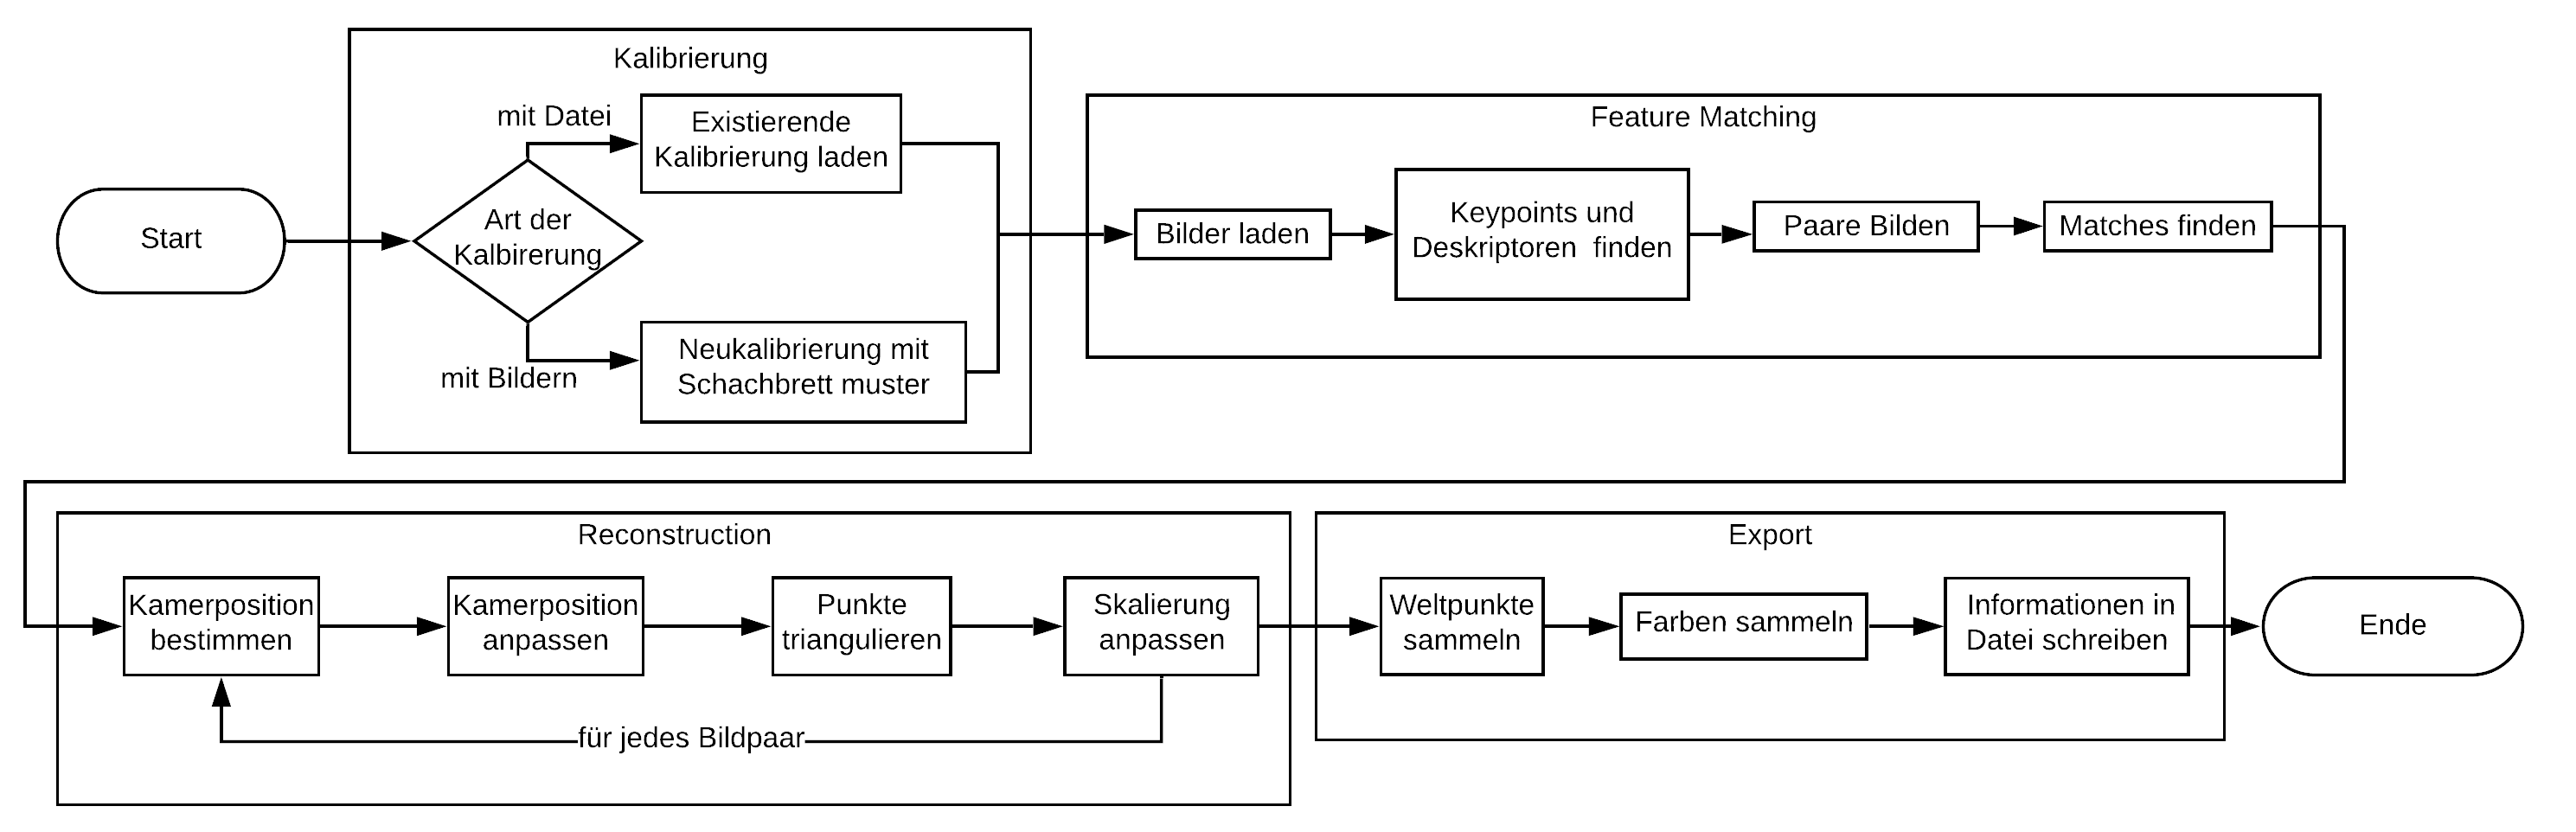
\includegraphics{src/img/konzept-pipeline.png}
    \caption{Rekonstruktierungspipline des Konzepts}
    \label{fig:concept-pipeline}
\end{figure}

% !TeX root = ../../main.tex
\ohead{Sebastian Schmitt}

\chapter{Umsetzung}
Im folgenden wird der Aufbau des Projektes sowie verwendete Bibliotheken erläutert.
Zusätzlich wird auf die Implementierung der einzelnen Schritte der SfM Pipeline eingegangen.

\section{Projektstruktur}
Die Applikation wird in C++ entwickelt.
Auch wenn Performance kein Ziel ist, wurde C++ gewählt um eine höhere Performance zu erreichen.
Einzige Abhängigkeit ist die offene Bibliothek OpenCV, siehe dazu \ref{sec:opencv}.
Zur Buildsteuerung wird das quelloffene Tool CMake verwendet.

Das Projekt ist folgendermaßen strukturiert:

\dirtree{%
.1 yapgt.
.2 include \ldots{} \begin{minipage}[t]{12cm}
Header-Dateien
\end{minipage}.
.2 resources \ldots{} \begin{minipage}[t]{12cm}
Bilder zum Testen von Kalibrierung und Feature-Matching
\end{minipage}.
.2 src \ldots{} \begin{minipage}[t]{12cm}
Implementierung
\end{minipage}.
.2 CMakeLists.txt \ldots{} \begin{minipage}[t]{12cm}
CMake Konfiguration
\end{minipage}.
}


\subsection{OpenCV}\label{sec:opencv}
Es wird OpenCV in der Version 4.2.0 mit dem Modul OpenCV Contrib verwendet.
OpenCV Contrib beinhaltet OpenCV Module, welche jedoch nicht stabil genug sind um Teil der offiziellen OpenCV Distribution zu sein \cite[README.md]{opencv_2013}.
OpenCV wurde mit folgenden Optionen kompiliert:
\begin{itemize}
	\item OPENCV\_EXTRA\_MODULES\_PATH um den Pfad zu OpenCV Contrib festzulegen
	\item OPENCV\_ENABLE\_NONFREE um auch nicht freie Algorithmen zu kompilieren
\end{itemize}
Auch wenn es Anforderung ist nur freie Bibliotheken zu verwenden, ist der Flag OPENCV\_ENABLE\_NON\_FREE notwendig.
Der in dieser Arbeit verwendete Algorithmus Scale-Invariant Feature Transform (SIFT) war bis 06. März 2020 von der University of British Columbia patentiert\footnote{siehe dazu https://patents.google.com/patent/US6711293} und ist daher in der verwendeten OpenCV Version nur mit OPENCV\_ENABLE\_NON\_FREE nutzbar.
SIFT ist Teil des Moduls Features2D extra (xfeatures2d) welches Teil von OpenCV Contrib ist und sowohl experimentelle als auch nicht freie Algorithmen beinhaltet.

Um die Applikation auch nutzen zu können ohne vorab OpenCV zu installieren oder zu kompilieren wurde CMake angewiesen, OpenCV statisch zu linken (siehe \autoref{lst:cmake_opencv_static}, Zeilen 1-4).
Zusätzlich kopiert CMake alle gelinkten Bibliotheken, auch wenn diesen nicht referenziert werden, in den Ausgabeordner, damit diese nicht von Hand kopiert werden müssen (\autoref{lst:cmake_opencv_static}, Zeilen 6-8).

\begin{lstlisting}[numbers=left, breaklines=true,breakatwhitespace=false,label=lst:cmake_opencv_static, caption=Ausschnitt von CMakeLists.txt um OpenCV statisch zu linken]
set(OPENCV_STATIC ON)
find_package(OpenCV REQUIRED)
[..]
target_link_libraries(yapgt ${OpenCV_LIBS})
[..]
foreach(CVLib ${OpenCV_LIBS})
    file(COPY ${_OpenCV_LIB_PATH}/${CVLib}${OpenCV_VERSION_MAJOR}${OpenCV_VERSION_MINOR}${OpenCV_VERSION_PATCH}d.dll DESTINATION ${CMAKE_BINARY_DIR})
endforeach()
\end{lstlisting}


\section{Kommandozeilenargumente}
Die einzelnen Schritte der Pipeline werden mittels Kommandozeilenargumente konfiguriert.
Zum Parsen der übergebenen Argumente wurde ein Argumentparser geschrieben.
Dieser ist in \emph{include/argparser.hpp} spezifiert und in \emph{src/argparser.c} implementiert.
Er beinhaltet den Namespace \emph{argparser} sowie zwei Klassen:
\begin{itemize}
\item \textbf{Argument}, repräsentiert ein Arguments (Name, Beschreibung, ob es übergeben wurde, welcher Wert übergeben wurde, ob es übergeben werden muss)
\item \textbf{ArgumentParser}, kennt alle Argumente, überprüft die übergebenen Argumente und legt fest ob und wie ein Argument übergeben wurde
\end{itemize}

Damit der \emph{ArgumentParser} auf Attribute von \emph{Argumenten} zugreifen darf, welche nicht öffentlich sein sollen, wurden diese als \emph{protected} markiert und \emph{ArgumentParser} innerhalb der Klasse \emph{Argument} als \emph{Friend Class} markiert (siehe dazu \autoref{lst:argparser_argument_friend}, Zeilen 2-3).
Auch wenn der übergebene Wert intern als String repräsentiert wird, kann er mit der Funktion \emph{getValue()} auch in andere primitive Typen konvertiert werden (\autoref{lst:argparser_argument_friend}, Zeilen 7-12).

\begin{lstlisting}[language=c++, numbers=left, breaklines=true, breakatwhitespace=false, label=lst:argparser_argument_friend]
namespace argparser {
    class Argument {
        friend class ArgumentParser;

    public:
        [..]
        template<typename T> T getValue() {
            std::istringstream in(this->value);
            T t = T();
            in >> t >> std::ws;
            return t;
        }
        [..]
    protected:
        std::string value;
        [..]
    };
    [..]
}
\end{lstlisting}

\begin{lstlisting}[language=c++, numbers=left, breaklines=true, breakatwhitespace=false, label=lst:argparser_example, caption=Argparser Verwendung]
int main(int argc, char *argv[]) {
    argparser::ArgumentParser parser("yapgt (yet another photogrammetry tool)");
    argparser::Argument a_loadCalibration("loadCalibration", "Filepath to load calibration from");    
    parser.addArgument(&a_loadCalibration);
    parser.parseArguments(argc, argv);
    if (a_loadCalibration.isFound()) {
        filesystem::path path(a_loadCalibration.getValue<string>());
    }
}
\end{lstlisting}

Der Argumentparser kann wie folgt benutzt werden:\\
Zunächst wird eine Instanz von \emph{ArgumentParser} erzeugt.
Als Parameter wird der Applikationsname übergeben.
Dieser wird beim Aufruf der Applikation mit dem Argument \emph{-help} angezeigt.
Danach wird ein Argument erzeugt.
Als Parameter werden der Name des Argumentes, sowie eine Beschreibung für Hilfe übergeben.
Danach wird das Argument dem ArgumentParser hinzugefügt.
Mit der Funktion \emph{parseArguments(argc, argv)} wird das eigentliche Verarbeiten der Argumente durchgeführt.
Mittels der Funktion \emph{isFound()} wird nun überprüft, ob das Argument übergeben wurde.
Der übergebene Wert kann nun mittels \emph{getValue<string>()} als String weiter verarbeitet werden.

\section{Kamera Kalibrierung}

\section{Feature Identifizierung}

\section{Feature Matching}

\section{Rekonstruktion}

\section{Export}
\subsection{PLY Format}
\subsection{Farben}
% !TeX root = ../../main.tex

\chapter{Testfälle}
\label{sec:testcases}
\ohead{Jan Maier}

In diesem Abschnitt wird die entwickelte Applikation in drei Testfällen getestet.
Die Testfälle sind dabei verschiedene Szenen mit mehreren Bildern von einem Objekt, das rekonstruiert werden soll.
Die Szenen und die Objekte sind dabei so gewählt, dass sie möglichst unterschiedlich sind in Bezug auf Größe und Beschaffenheit des Objekts.
In jedem Testfall wird die Szene kurz beschrieben und die Qualität der Feature Matches, sowie ihre rekonstruierten Punkte bewertet.
Bei der Bewertung wird zu einem auf die Beschaffenheit der Szene und des Objekts und zum anderem auf die Implementierung eingegangen.
In XXX werden die Ergebnisse der Testfälle zusammengefasst.

\section{Fall 1: Sessel}
\label{sec:textcase-chair}\ohead{Jan Maier}
Im ersten Testfall wird versucht einen Sessel zu rekonstruieren.
Dazu werden 10 Bilder verwendet, welche den Sessel aus verschiedenen Winkeln zeigt.
Die Bilder sind so sortiert, dass die Bewegung zwischen zwei Bildern minimal ist.
Die Anzahl der Matches, der rekonstruierten Punkte, sowie die Anzahl der Weltpunkte, die für die Skalierung genutzt wurden, so wie Skalierung selbst werden in \cref{tab:chair-results} gezeigt. % TODO: rewording
Das erste Bildpaar des Sessels wird in \cref{fig:chair-first-pair} gezeigt.
In \cref{fig:chair-first-pair-with-matches} wird das selbe Bildpaar mit allen Keypoints und ihren Matches gezeigt.
Matches sind dabei durch Linien gekennzeichnet, die die korrespondierenden Bildpunkte miteinander verbinden.
Hier fällt auf, dass sich die Matches überwiegend auf den Seiten des Sessels befinden.
Auch der Text auf der Decke und dem Kissen, so wie das karierte Muster des anderen Kissens werden als Keypoints erkannt und gematcht. % todo: rewording.
Des Weiteren sind viele Keypoints und Matches auf dem Teppich unten im Bild zu erkennen.
Im Gegensatz dazu gibt es sehr wenige Matches auf dem Boden, der Heizung, der Wand, sowie auf der Decke und dem Sitzkissen des Sessels.
Dies liegt daran, dass diese Texturen keine Kanten besitzen, die von den Feature Extractor als Feature erkannt werden können.
Dementsprechend fehlen diese Flächen bei den rekonstruierten Punkten, wie in \cref{fig:chair-model} zu sehen ist.  
Die generelle Form des Sessels und der Kissen ist in dem Modell gut zu erkennen.
Von der Decke ist nur ein streifen zu sehen, wo Matches an dem Text existieren.  
Das Sitzkissen ist überhaupt nicht zu sehen.
In \cref{fig:chair-model-2} ist das Modell von der anderen Seite und einem höheren Blickwinkel zu sehen.
Hier sind mehrere Punktsammlungen zusehen, die das gleiche darstellen, aber verschoben sind.
So etwa die Vorderseite und die Kissen des Sessels.
Dies lässt eine ungenaue Skalierung des Translationsvektors vermuten.

\begin{table}
    \begin{tabularx}{\textwidth}{cXXXX}
        \toprule
        Bildpaar &  Anzahl der Matches & Anzahl der Weltpunkte & Anzahl der Weltpunkte für Skalierung
 & angewandte Skalierung \\ 
        \midrule
        1 & 1.570 & 1.569 & -  & - \\
        2 & 1.548 & 1.548 & 522 & 1,15455 \\
        3 & 1.405 & 1.404 & 494 & 1,09323 \\
        4 & 1.550 & 1.550 & 535 & 1,0002 \\
        5 & 1.426 & 1.413 & 658 & 0,796158 \\
        6 & 1.196 & 1.187 & 623 & 1,14341 \\
        7 & 923 & 918 & 372 & 0,523695 \\
        8 & 744 & 721 & 248 & 1,18605 \\
        9 & 1.352 & 1.351 & 241 & 0,851274 \\
        \midrule
        Summe & 11.714 & 11.661 & 3.693 & - \\
        \bottomrule
    \end{tabularx}
    \caption{XX}
    \label{tab:chair-results}
\end{table}

\begin{figure}
    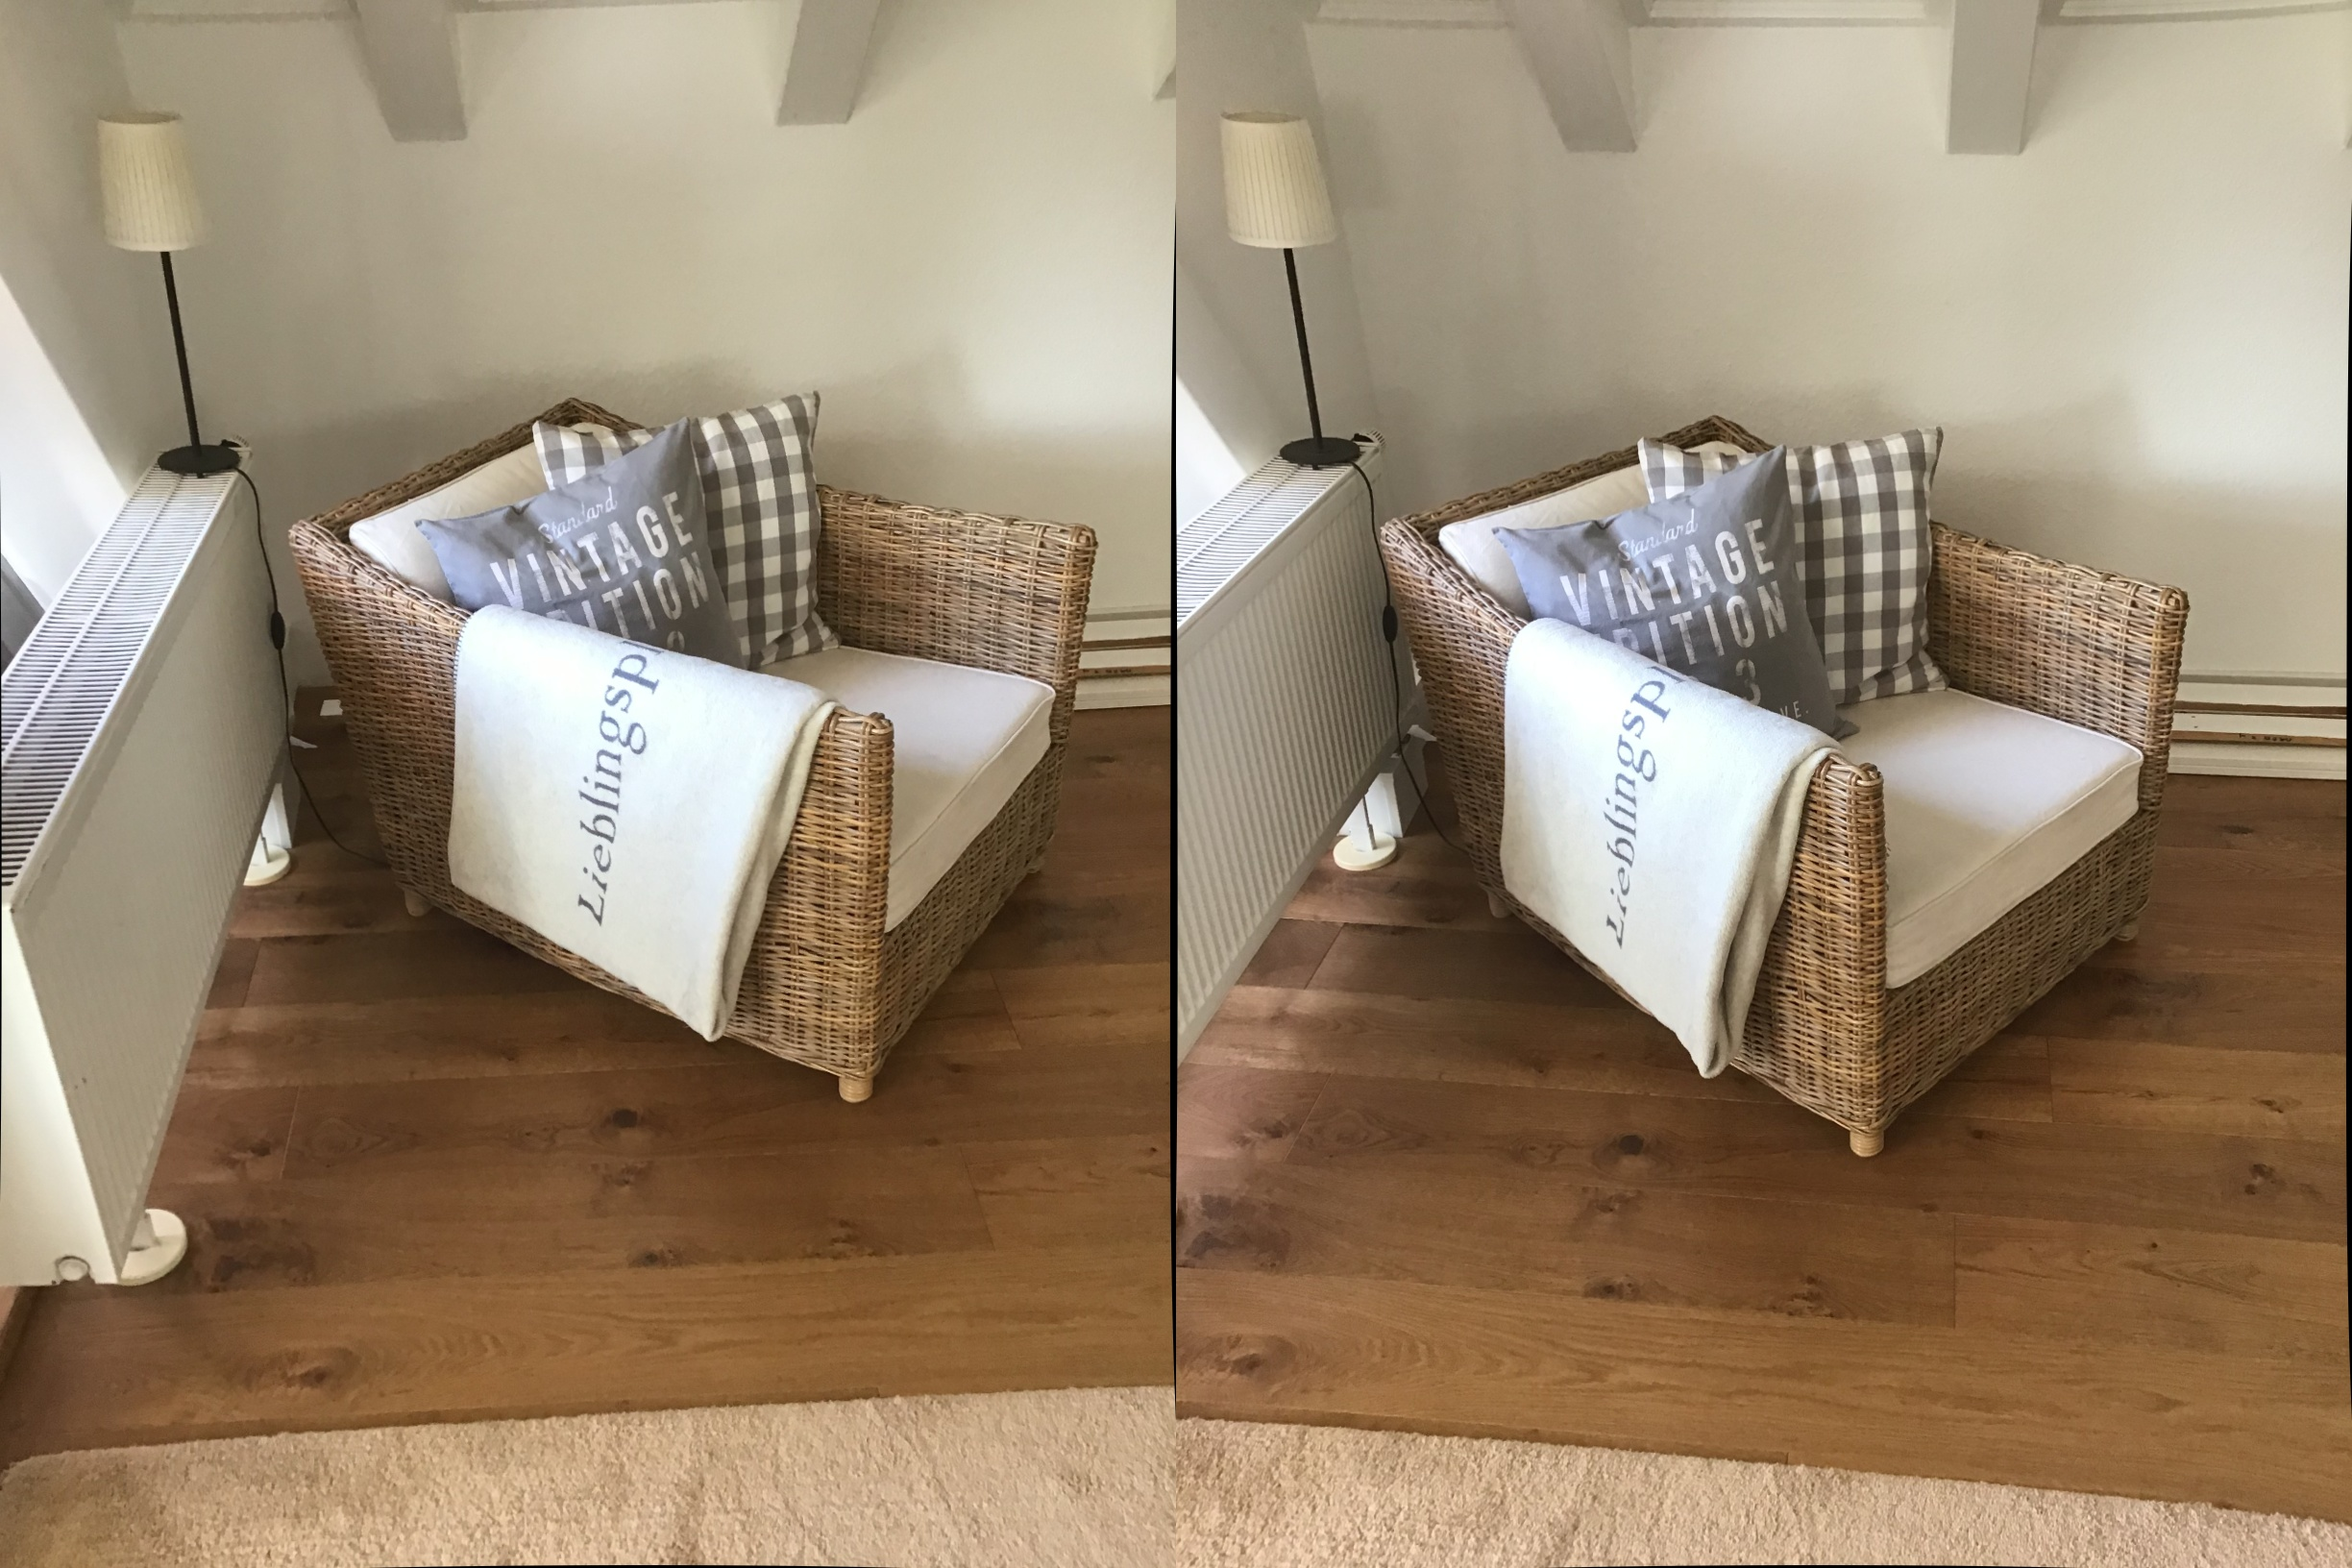
\includegraphics[width=\textwidth]{src/img/chair_first_pair.jpg}
    \caption{Eins von zehn Bildpaaren zum Rekonstruieren des Sessels.}
    \label{fig:chair-first-pair}
\end{figure}

\begin{figure}
    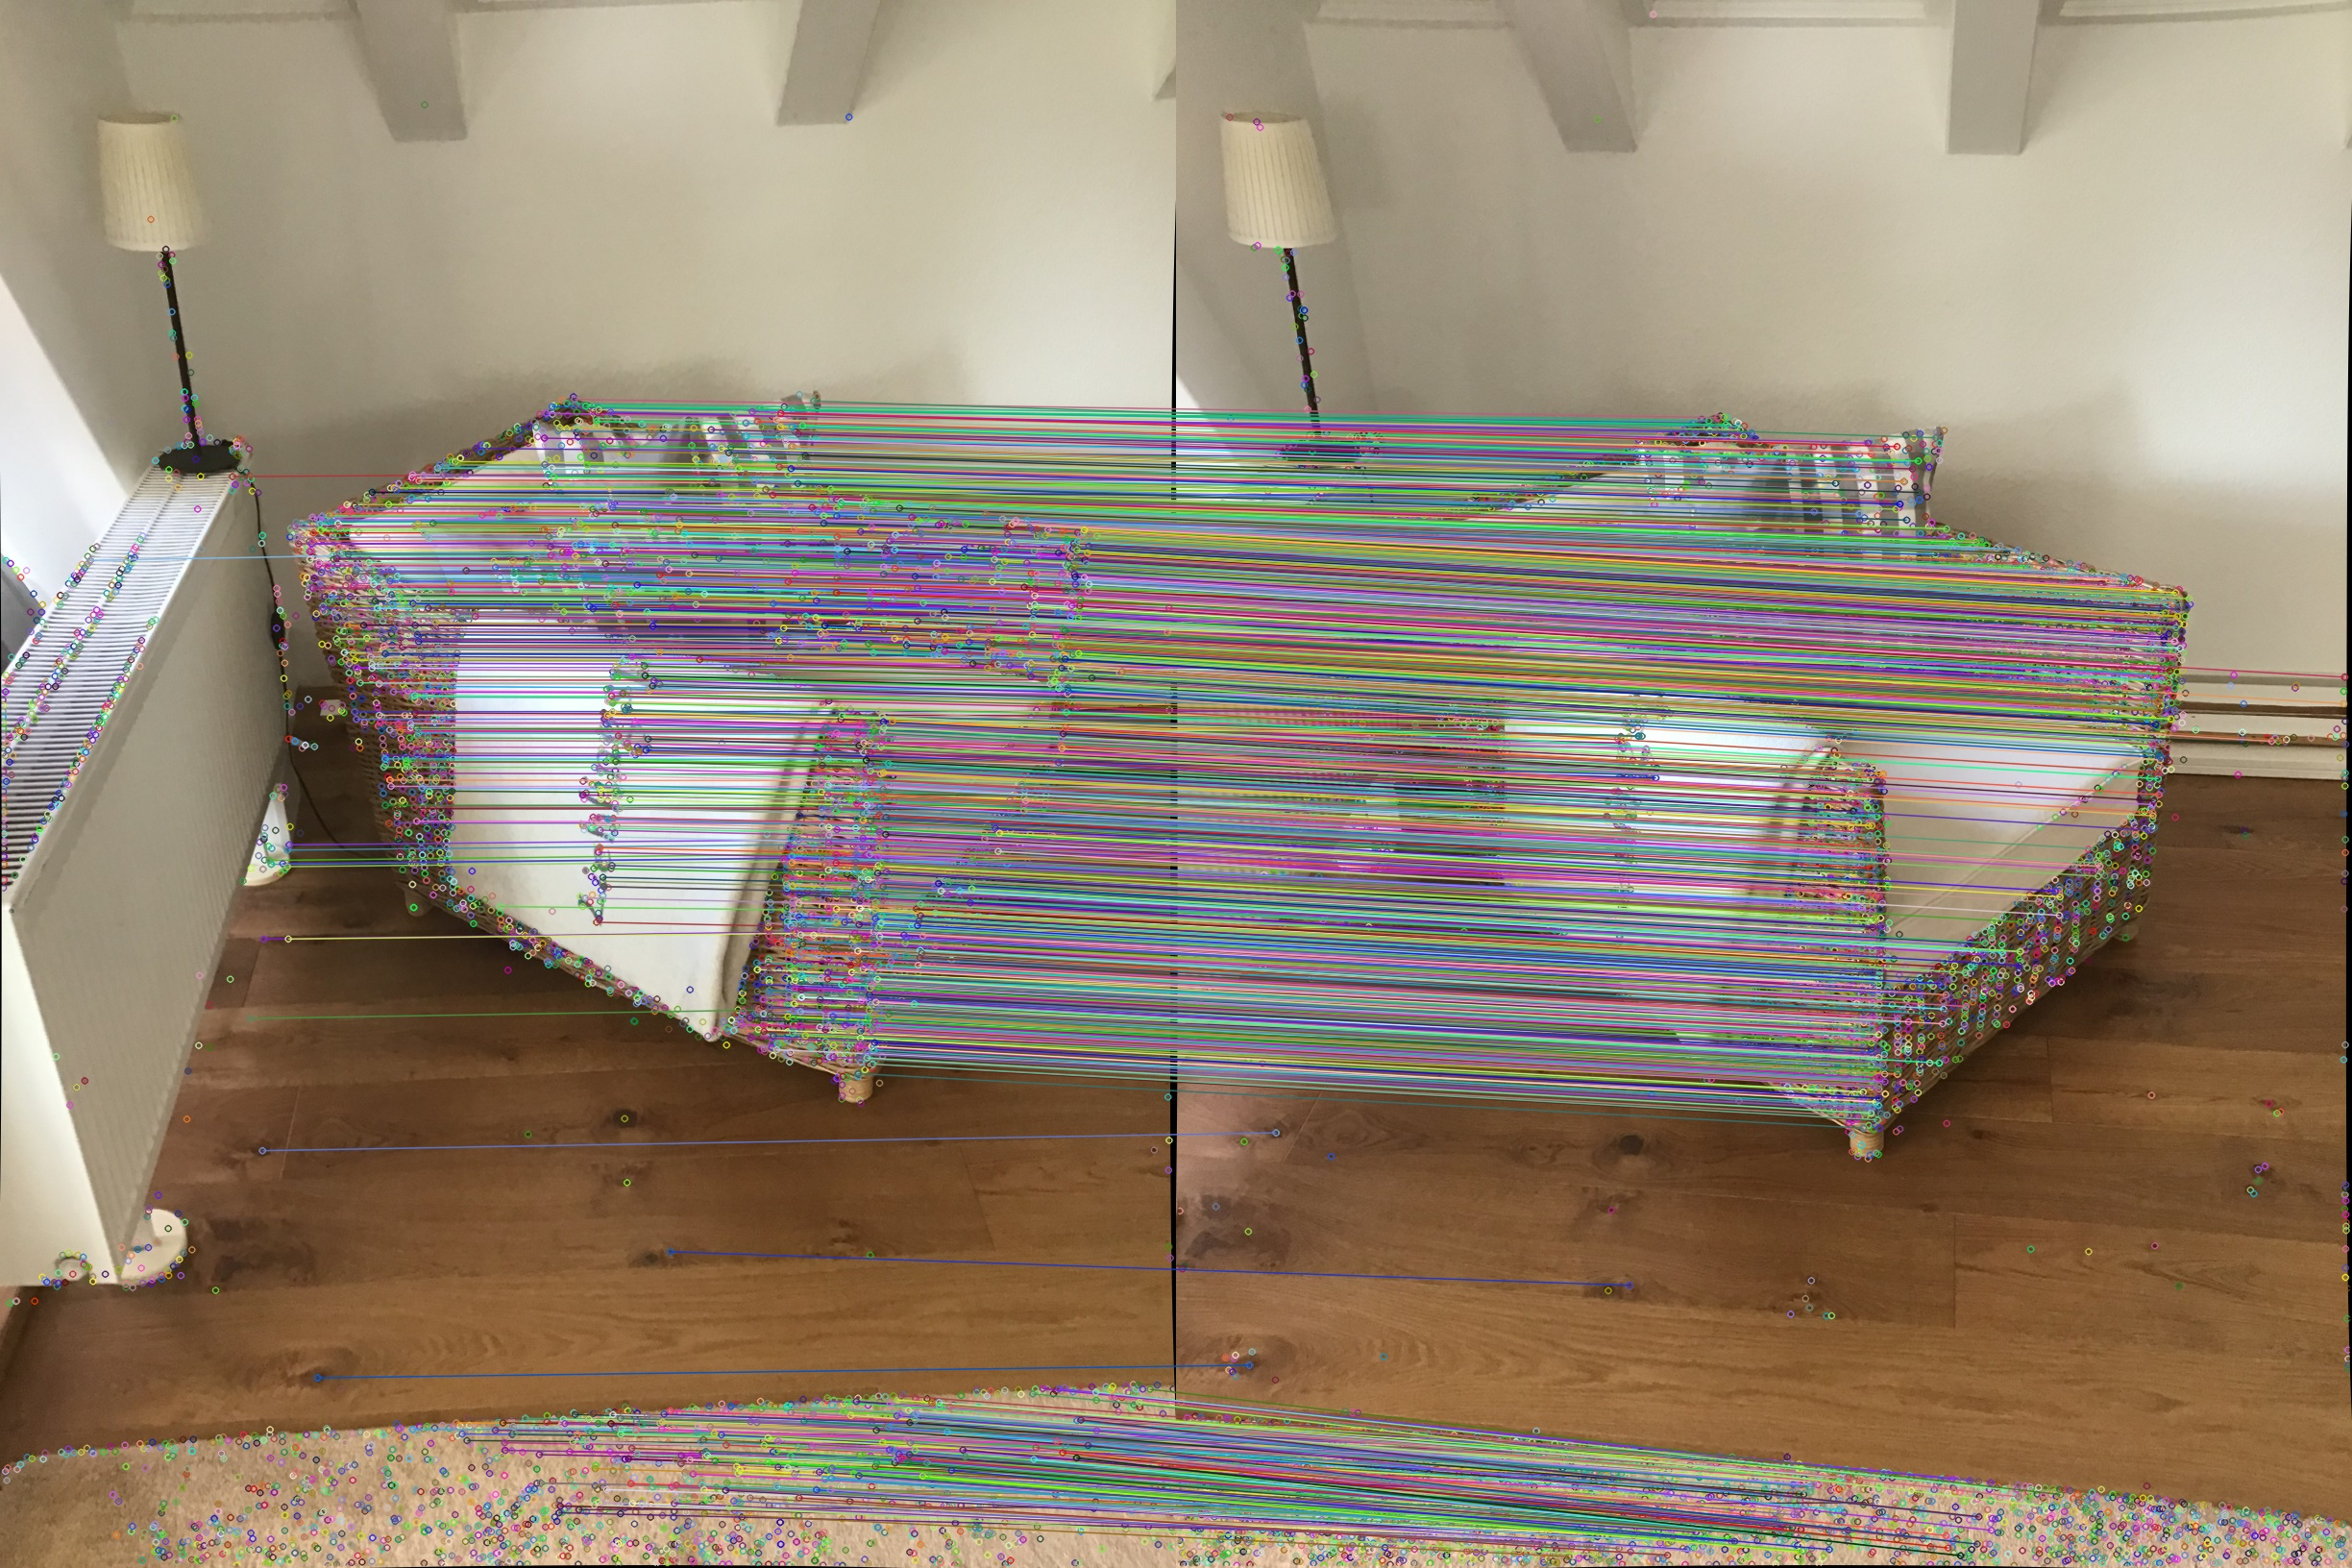
\includegraphics[width=\textwidth]{src/img/chair_first_pair_with_matches.jpg}
    \caption{Bildpaar des Sessels mit Keypoints und Matches.}
    \label{fig:chair-first-pair-with-matches}
\end{figure}

\begin{figure}
    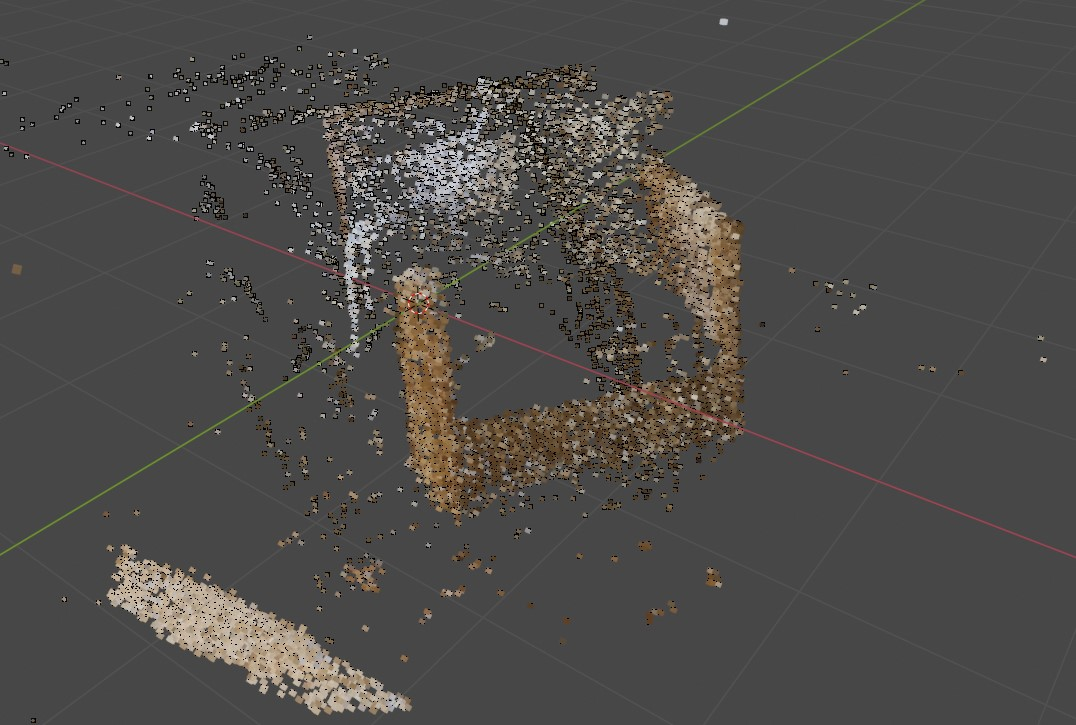
\includegraphics[width=\textwidth]{src/img/chair_model.jpg}
    \caption{Die rekonstruierten Bildpunkte des Sessels in Blender. Das Modell wurde um -119 Grad um die X gedreht, sowie um -4.8 Meter in Y und 2.7 Meter in Z Richtung verschoben.}
    \label{fig:chair-model}
\end{figure}

\begin{figure}
    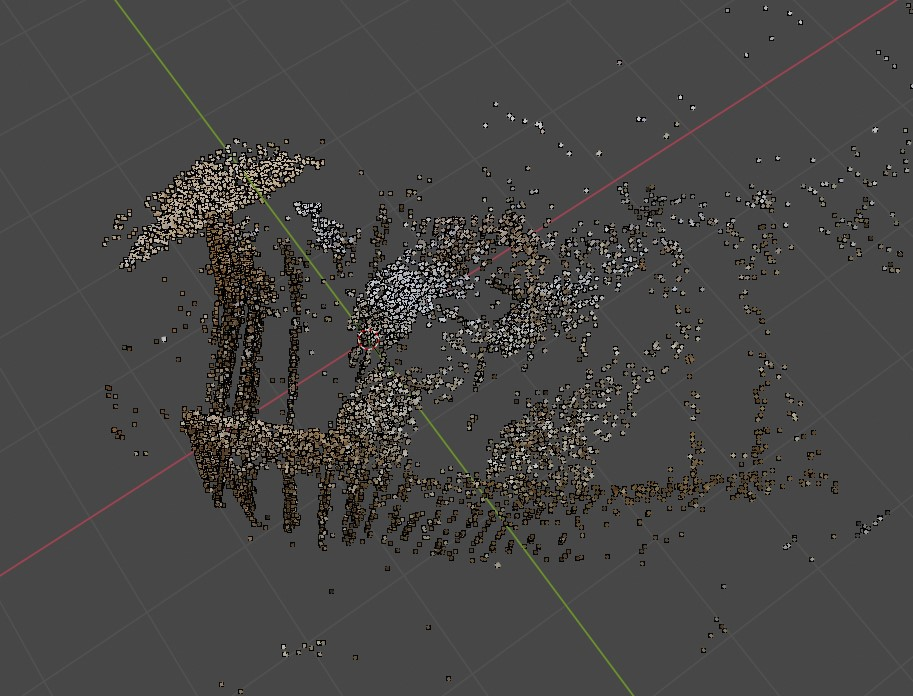
\includegraphics[width=\textwidth]{src/img/chair_model_2.jpg}
    \caption{Das Sessel Modell in einem anderem Blickwinkel}
    \label{fig:chair-model-2}
\end{figure}


\section{Fall 2: Auto}
\label{sec:textcase-car}
Im zweiten Testfall wird die Rekonstruktion eines Autos getestet. 
Insgesamt wurden 17 Bilder von einem schwarzen Skoda Fabia gemacht, die das Auto in verschiedenen Positionen zeigt.
Die Tabelle~\cref{tab:car-results} zeigt Anzahl der rekonstruierten Punkte pro Bildpaar.
Im Vergleich zum ersten Testfall gibt es hier deutlich weniger Matches, rekonstruierte Punkte und Punkte,die für die Skalierung verwendet worden sind.
\cref{fig:car-second-pair,fig:car-second-pair-with-matches} zeigen das zweite Bildpaar vom Auto.
Hier ist sehen, dass dass die Keypoints der meisten Matches nicht auf auf dem Auto liegen.
Statt dessen werden Matches eher an den Wänden, Pflanzen und auf dem Boden gefunden.
Bei dem Auto selbst werden die Matches hauptsächlich nur am Nummernschild und vereinzelt in den Reflexionen der Umgebung gefunden.
Wie durch die schlechten Matches zu erwarten ist, kann das Auto in den rekonstruierten Modell nicht erkannt werden, wie in \cref{fig:car-model} zu sehen ist.
In \cref{fig:car-model-2} ist das Modell aus einem anderem Winkel zu sehen.
Hier ist deutlich zu erkennen, dass die grünen Punkte der Pflanzen im Hintergrund in der gleichen Ebene wie viele Andere Punkte liegen. 
Dies lässt auf einen Fehler in der Triangulation oder Skalierung der Punkte vermuten.

\begin{table}
    \begin{tabularx}{\textwidth}{c r r r r}
        \toprule
        Bildpaar &  Anzahl der Matches & Anzahl der Weltpunkte & Anzahl der Überlappende Weltpunkte & angewandte Skalierung \\ 
        \midrule
        1  & 575 & 480 & -  & - \\
        2  & 910 & 860 & 165 & 0,468641 \\
        3  & 685 & 653 & 227 & 0,768563 \\
        4  & 583 & 570 & 51  & 0,788242 \\
        5  & 264 & 247 & 25  & 0,60277 \\
        6  & 427 & 409 & 58  & 0,848896 \\
        7  & 393 & 346 & 95  & 2,80038 \\
        8  & 799 & 527 & 99  & 0,923119 \\
        9  & 827 & 518 & 113 & 0,577807 \\
        10 & 618 & 597 & 125 & 1,11263 \\
        11 & 251 & 187 & 56  & 0,472208 \\
        12 & 68  & 36  & 10  & 1,49154 \\
        13 & 341 & 325 & 2   & 1,33112 \\
        14 & 334 & 263 & 18  & 2,02715 \\
        15 & 175 & 166 & 12  & 0,475839 \\
        16 & 167 & 146 & 21  & 0,651284 \\
        \midrule
        Summe & 7.417 & 6.330 & 1.077 & - \\
        \bottomrule
    \end{tabularx}
    \caption{Ergebnis der Rekonstruktion der Autobilder.}
    \label{tab:car-results}
\end{table}

\begin{figure}
    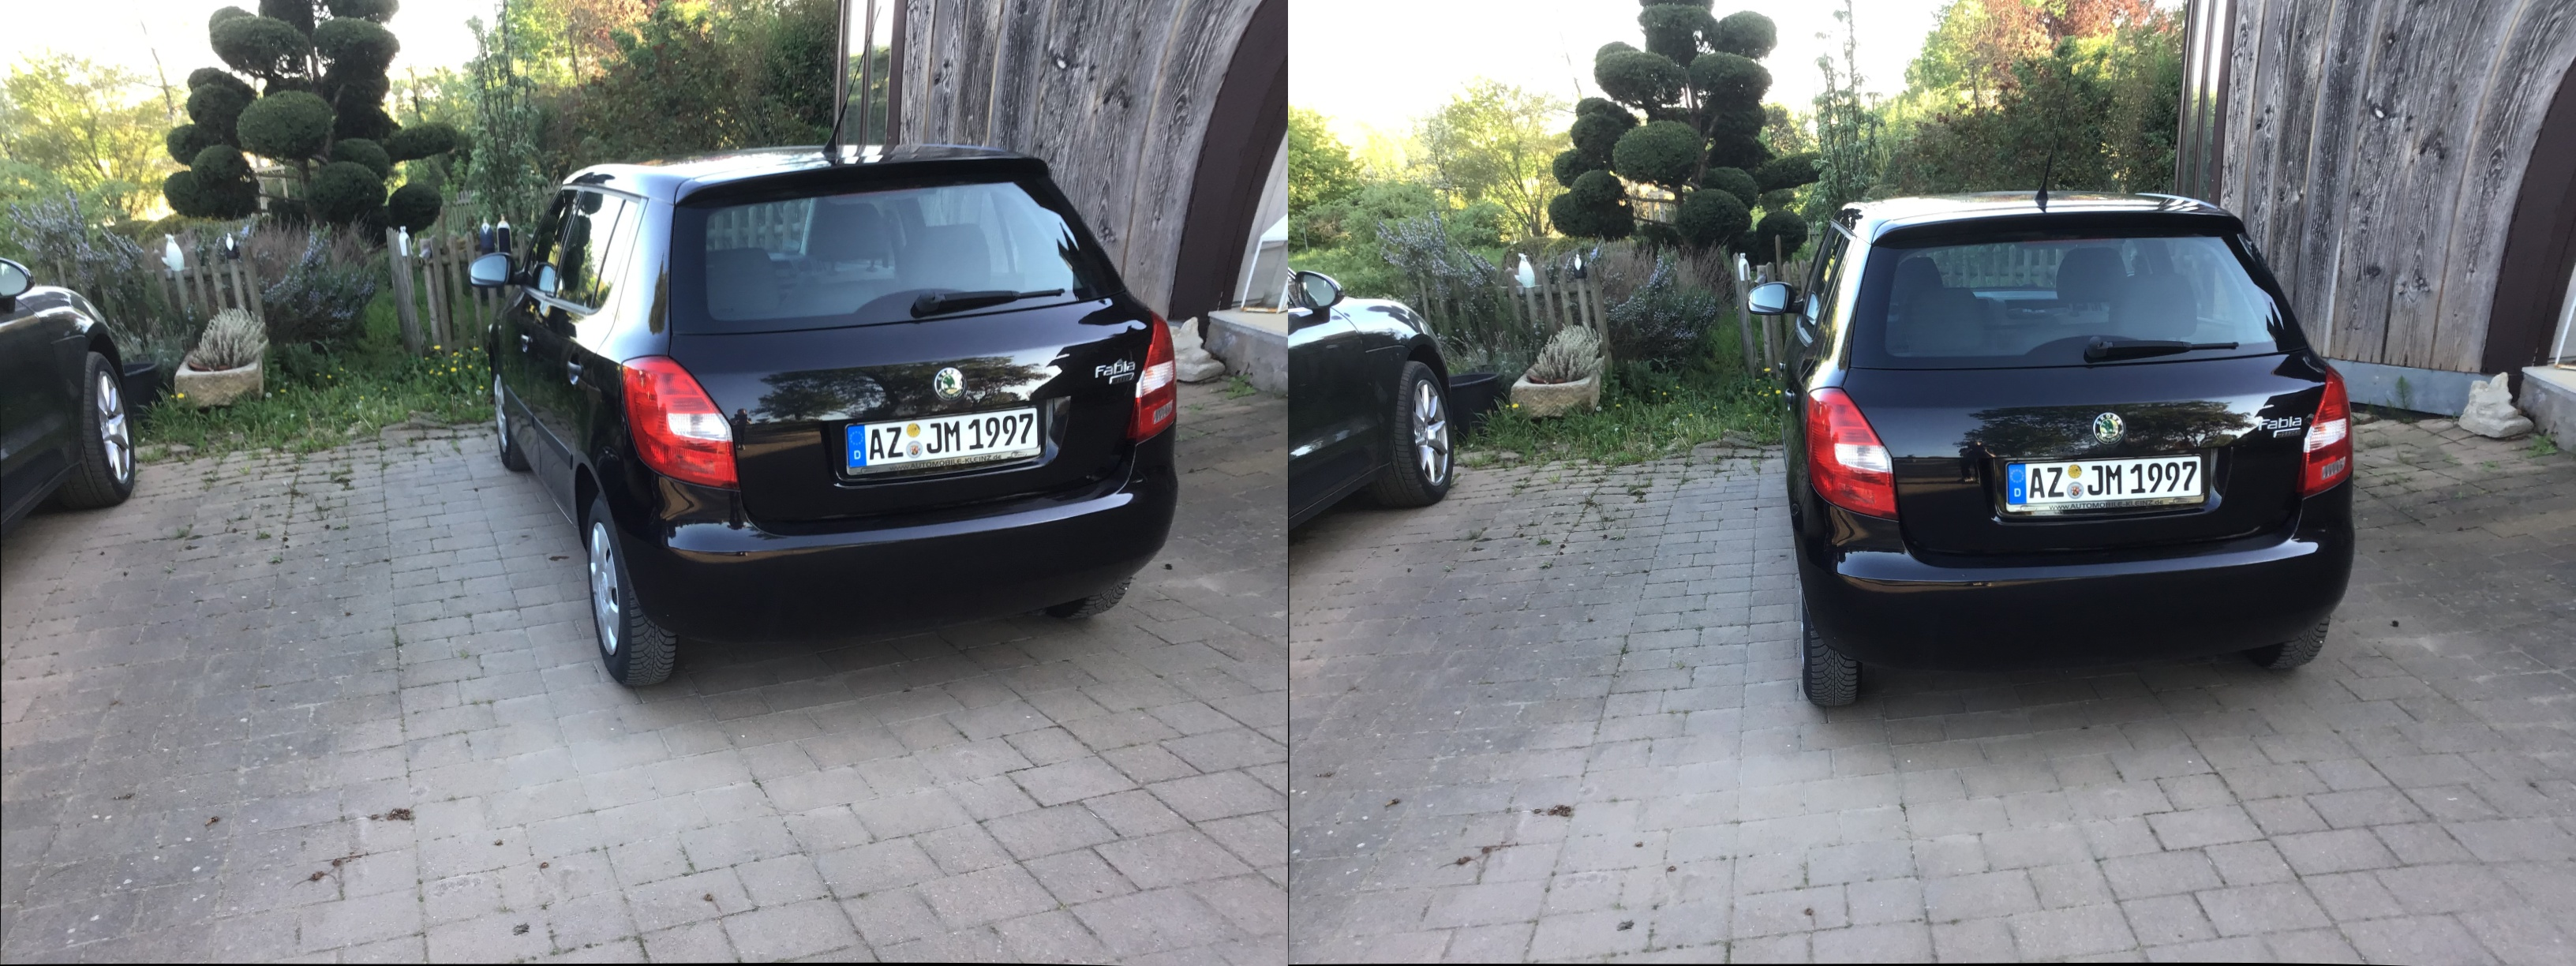
\includegraphics[width=\textwidth]{src/img/car_second_pair.jpg}
    \caption{Das zweite Bildpaar zum Rekonstruieren des Autos.}
    \label{fig:car-second-pair}
\end{figure}

\begin{figure}
    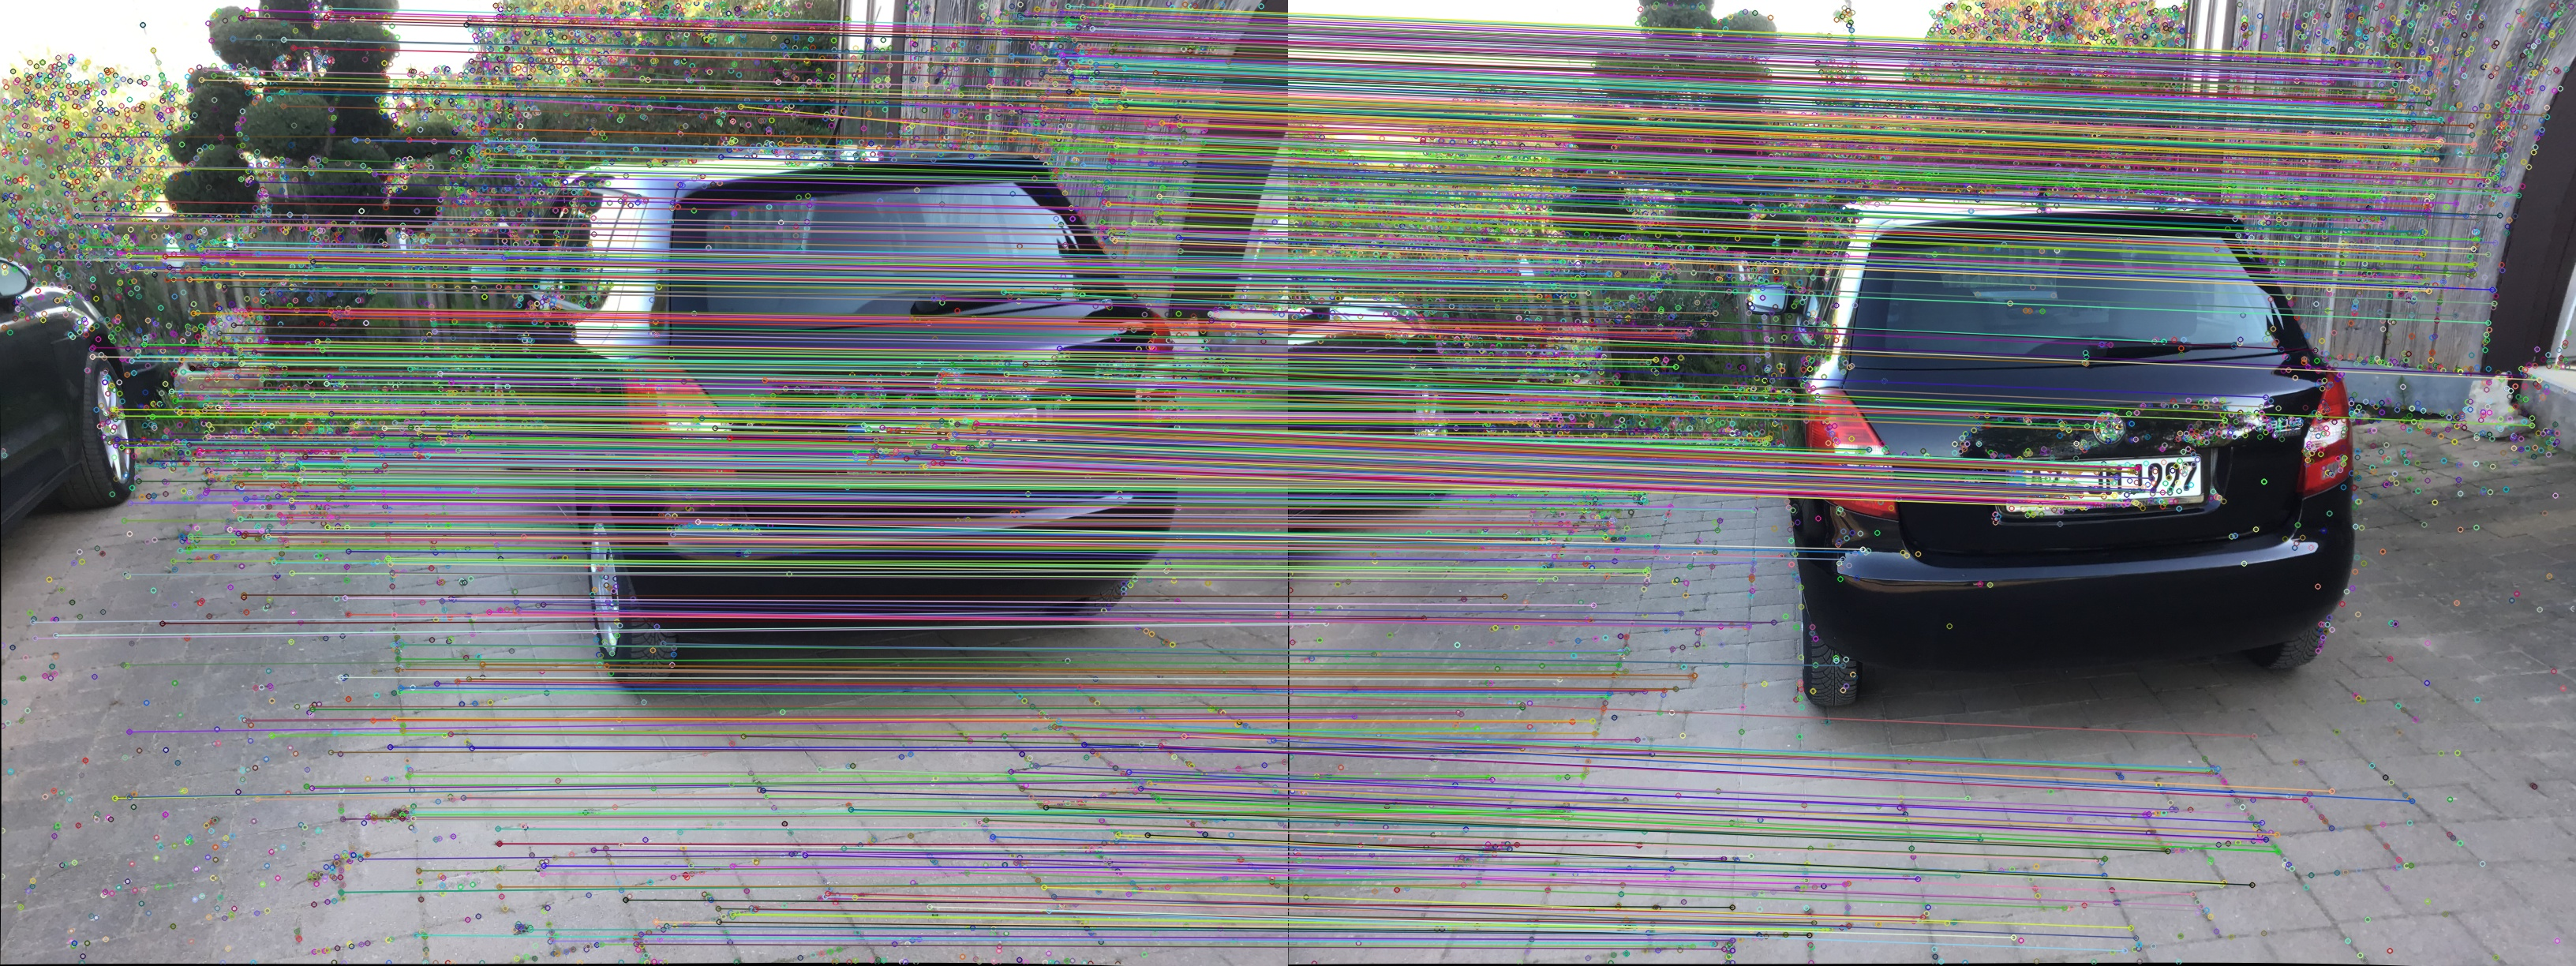
\includegraphics[width=\textwidth]{src/img/car_second_pair_with_matches.jpg}
    \caption{Das zweite Bildpaar vom Auto mit Keypoints und Matches.}
    \label{fig:car-second-pair-with-matches}
\end{figure}

\begin{figure}
    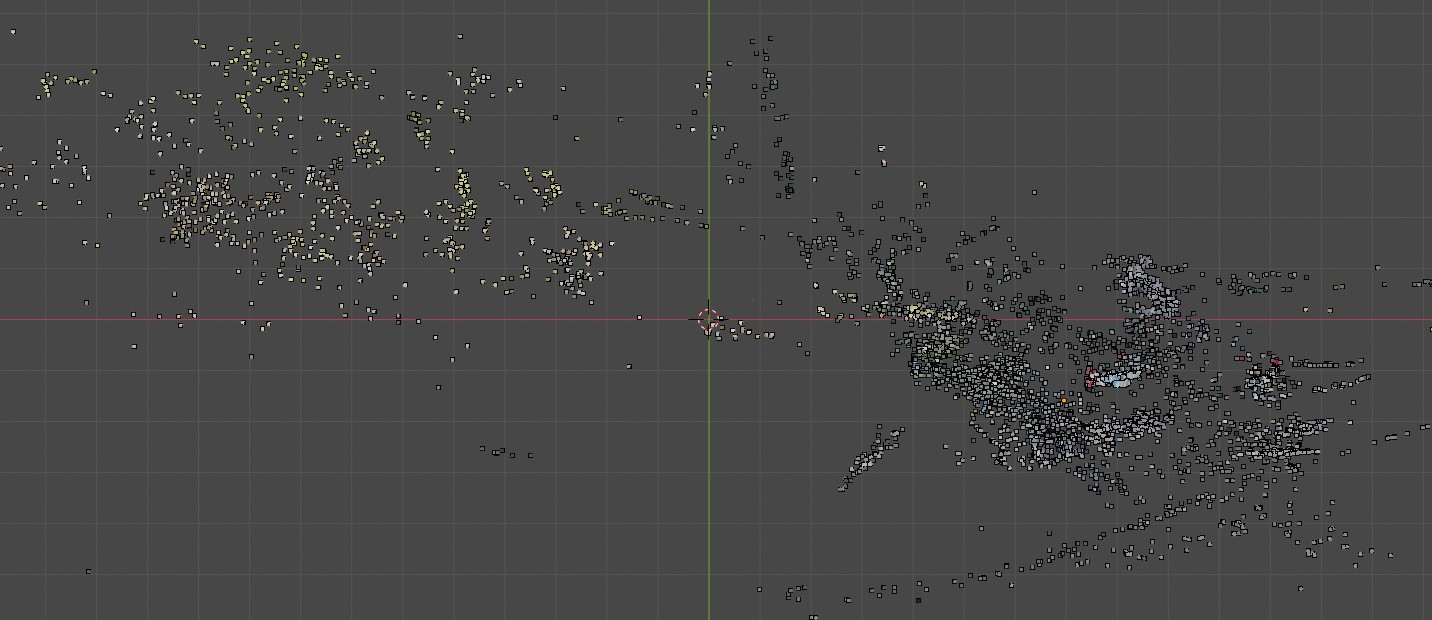
\includegraphics[width=\textwidth]{src/img/car_model.jpg}
    \caption{Das zweite Bildpaar vom Auto mit Keypoints und Matches.}
    \label{fig:car-model}
\end{figure}

\begin{figure}
    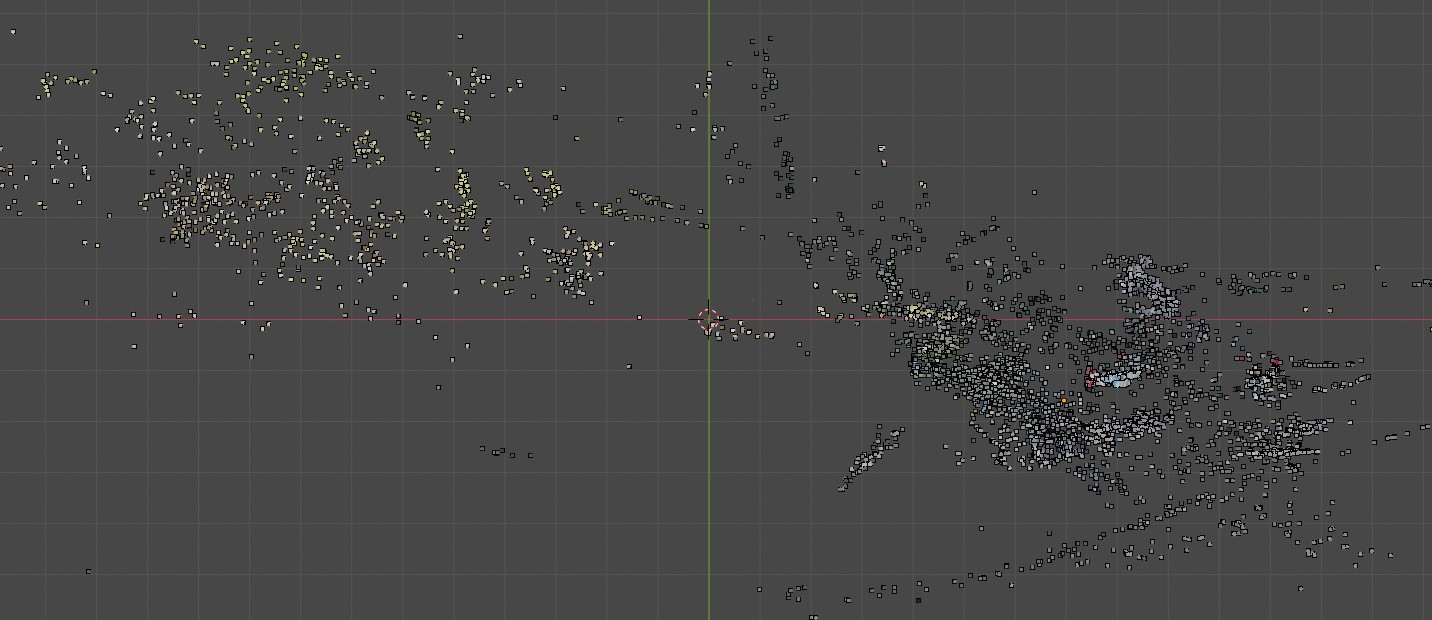
\includegraphics[width=\textwidth]{src/img/car_model.jpg}
    \caption{Das zweite Bildpaar vom Auto mit Keypoints und Matches.}
    \label{fig:car-model-2}
\end{figure}

\section{Fall 3: Hund}
\label{sec:testcase-dog}
Im dritten Testfall wird versucht mit neuen Bildern einen Hund in einem Körbchen zu rekonstruieren, der in \cref{fig:dog-image} zu sehen ist.

Die \cref{tab:dog-results} zeigt die Ergebnisse der Rekonstruktion.
In allen Bildpaaren ist der Matches höher als im ersten Testfall.
Betracht man jedoch in \cref{fig:dog-first-pair-with-matches} wo die Matches liegen, dann fällt auf, dass keine auf dem Hund liegen.
Stattdessen befinden sich alle Matches auf dem Teppich.
Das Modell in Blender zeigt dem entsprechend nur eine Fläche, die aus beige Punkten besteht.
Das Problem in diesem Testfall ist wie beim Auto und dem Sitzkissen des Sessels, dass der Hund keine auffälligen Kanten besitzt, die als Feature erkannt werden.
Des Weiteren ist das Aufnehmen der Fotos in diesem Fall problematisch. 
Im Vergleich zum Sessel oder dem Auto ist es schwierig mehrere und gute Bilder von dem Hund zu machen, ohne dass er sich bewegt. 
Es war nicht möglich den Hund stehend zu fotografieren, da er entweder weiter gelaufen ist oder den Kopf mit der Kamera bewegt hat.
Die Fotos konnten erst dann gemacht werden, wenn der Hund zufällig im Körbchen gelegen hat und sich nicht beweg hat.

\begin{figure}
    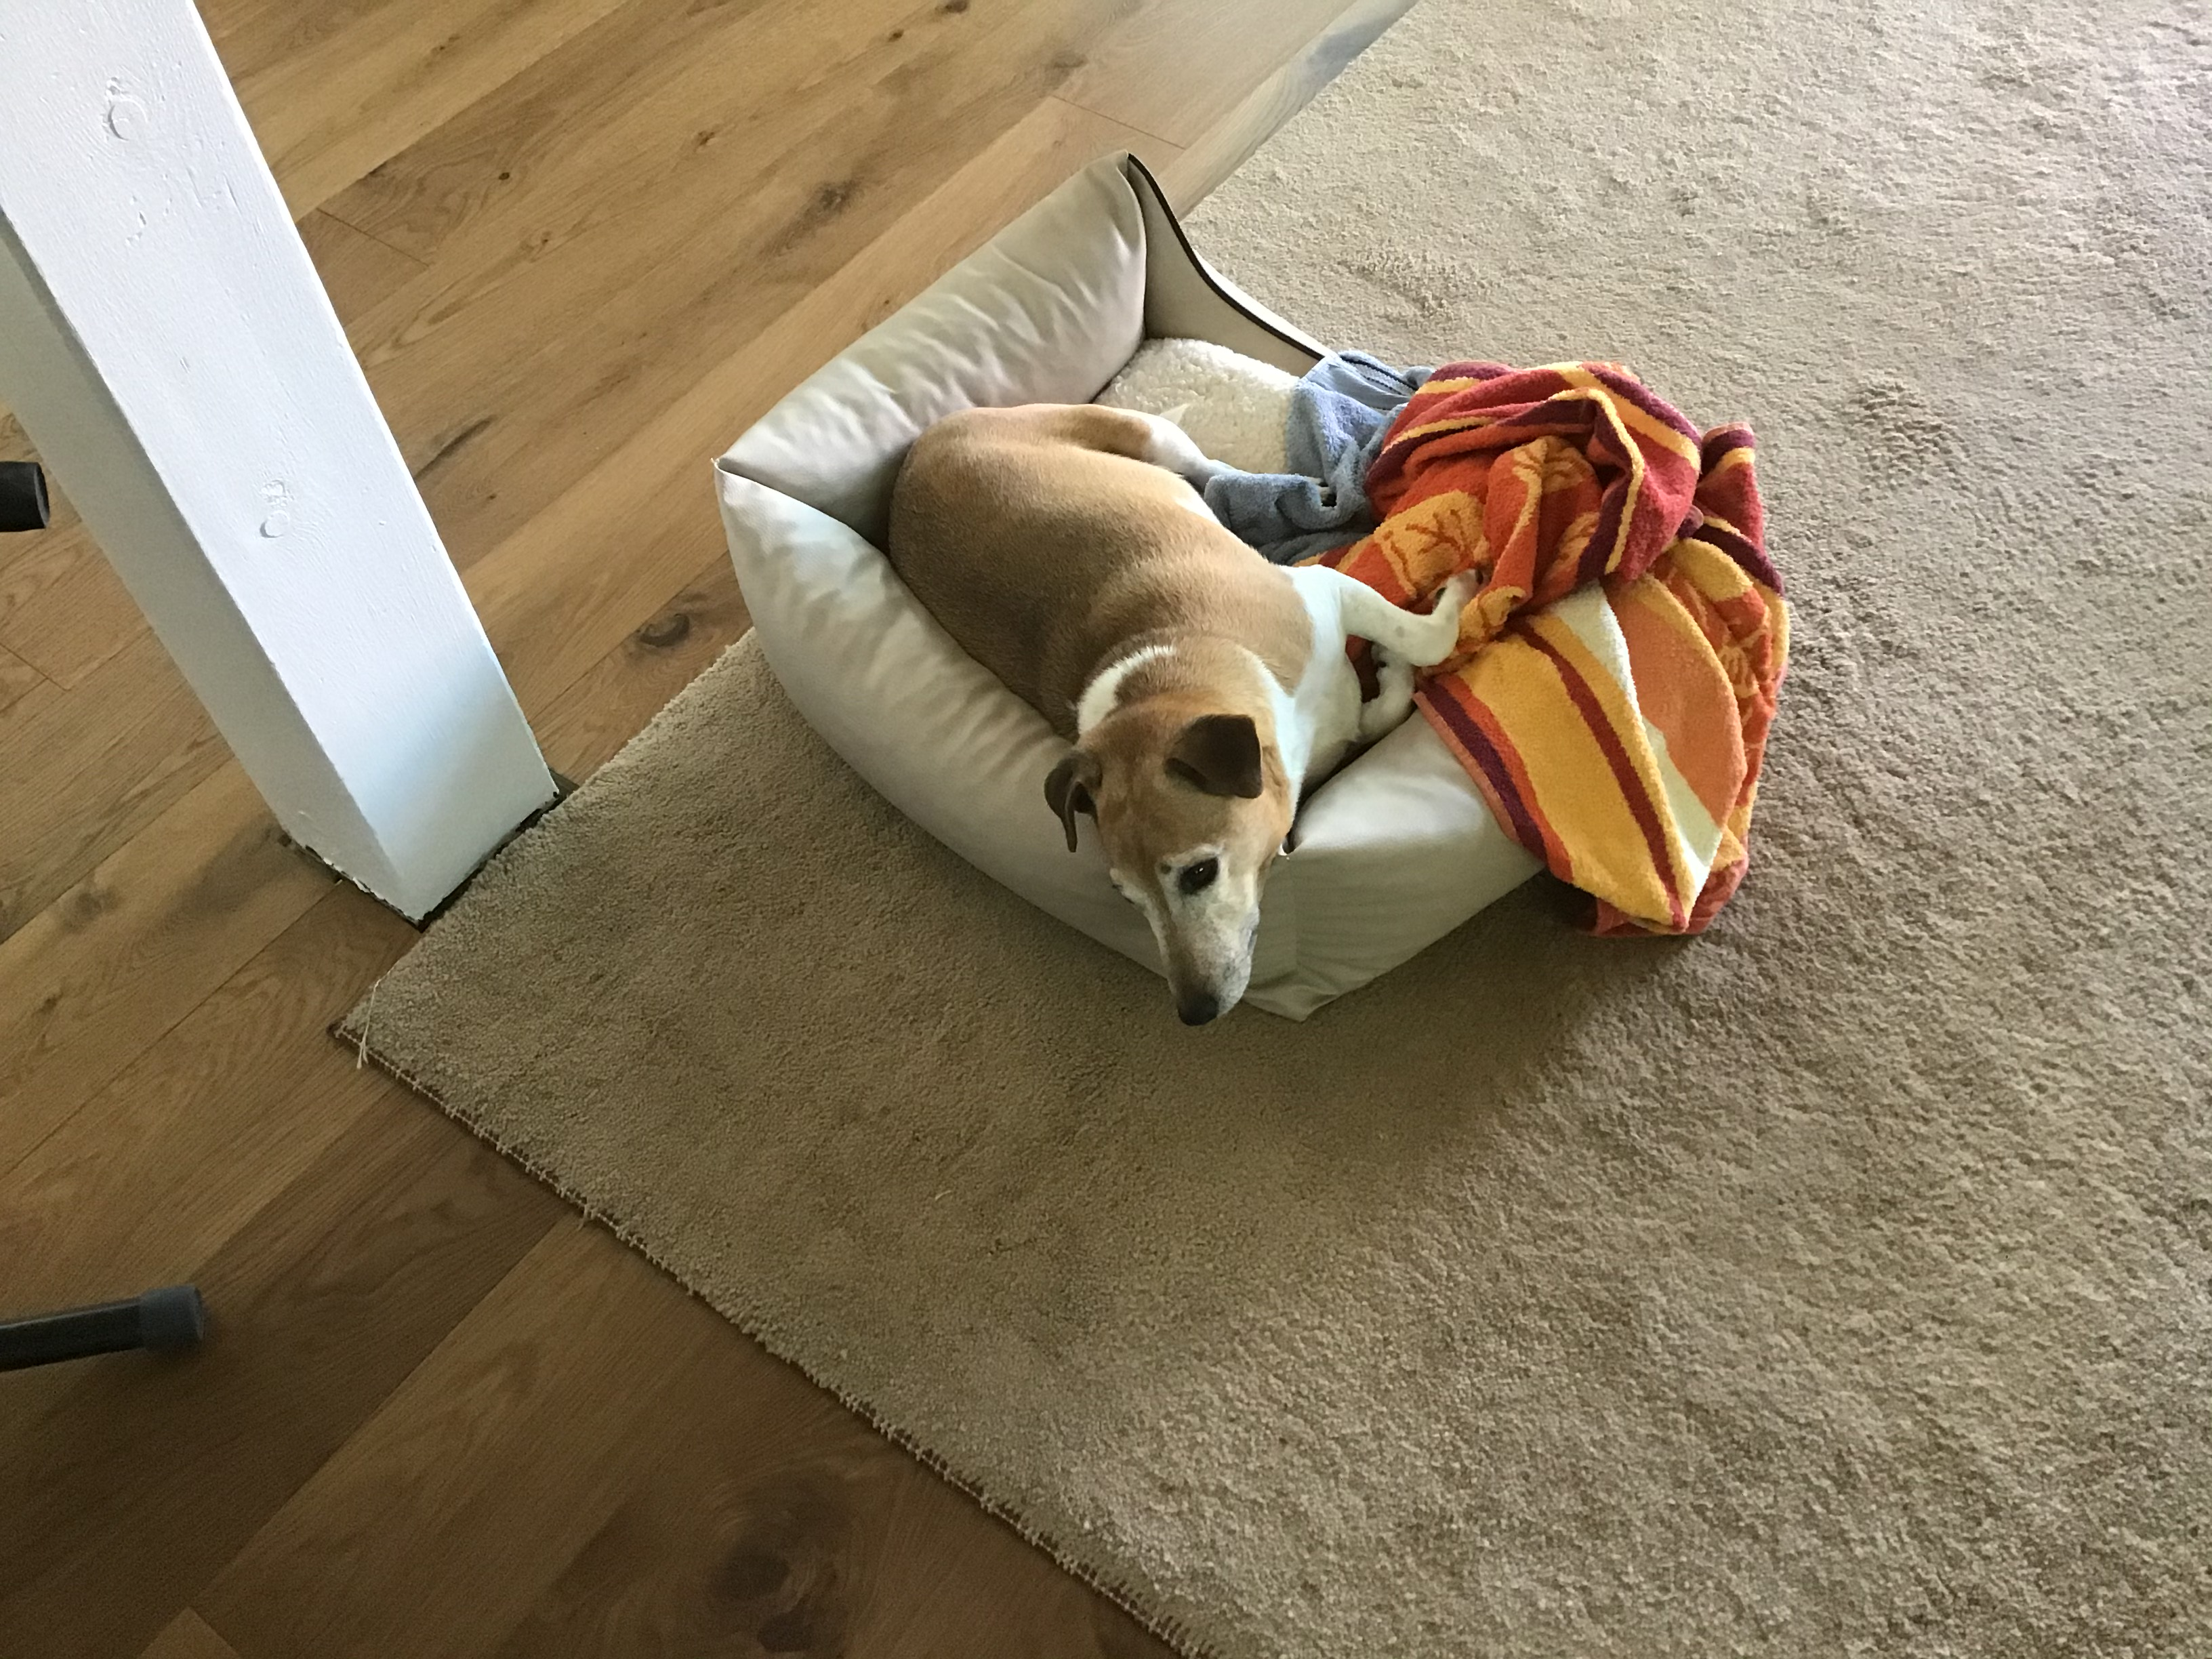
\includegraphics[width=\textwidth]{src/img/dog.jpg}
    \caption{Der Hund, genannt Sam, der im Körbchen liegt und rekonstruiert wird.}
    \label{fig:dog-image}
\end{figure}

\begin{table}
    \begin{tabularx}{\textwidth}{cXXXX}
        \toprule
        Bildpaar &  Anzahl der Matches & Anzahl der Weltpunkte & Anzahl der Weltpunkte für Skalierung & angewandte Skalierung \\ 
        \midrule
        1 & 4.799 & 4.786 & -  & - \\
        2 & 6.450 & 6.421 & 2.127 & 0,835131 \\
        3 & 6.525 & 6.472 & 2.763 & 0,892978 \\
        4 & 7.520 & 7.489 & 2.867 & 0,975344 \\
        5 & 7.462 & 7.444 & 3.215 & 0,801014 \\
        6 & 3.024 & 2.984 & 1.651 & 0,93856  \\
        7 & 6.071 & 6.009 & 1.337 & 1,42251  \\
        8 & 7.893 & 7.874 & 3.091 & 0,707064 \\
        9 & 6.917 & 4.350 & 1.924 & 1,01307  \\
        \midrule
        Summe & 56.661 & 53.829 & 18.975 & - \\
        \bottomrule
    \end{tabularx}
    \caption{Ergebnis der Rekonstruktion der neun Hundebilder}
    \label{tab:dog-results}
\end{table}

\begin{figure}
    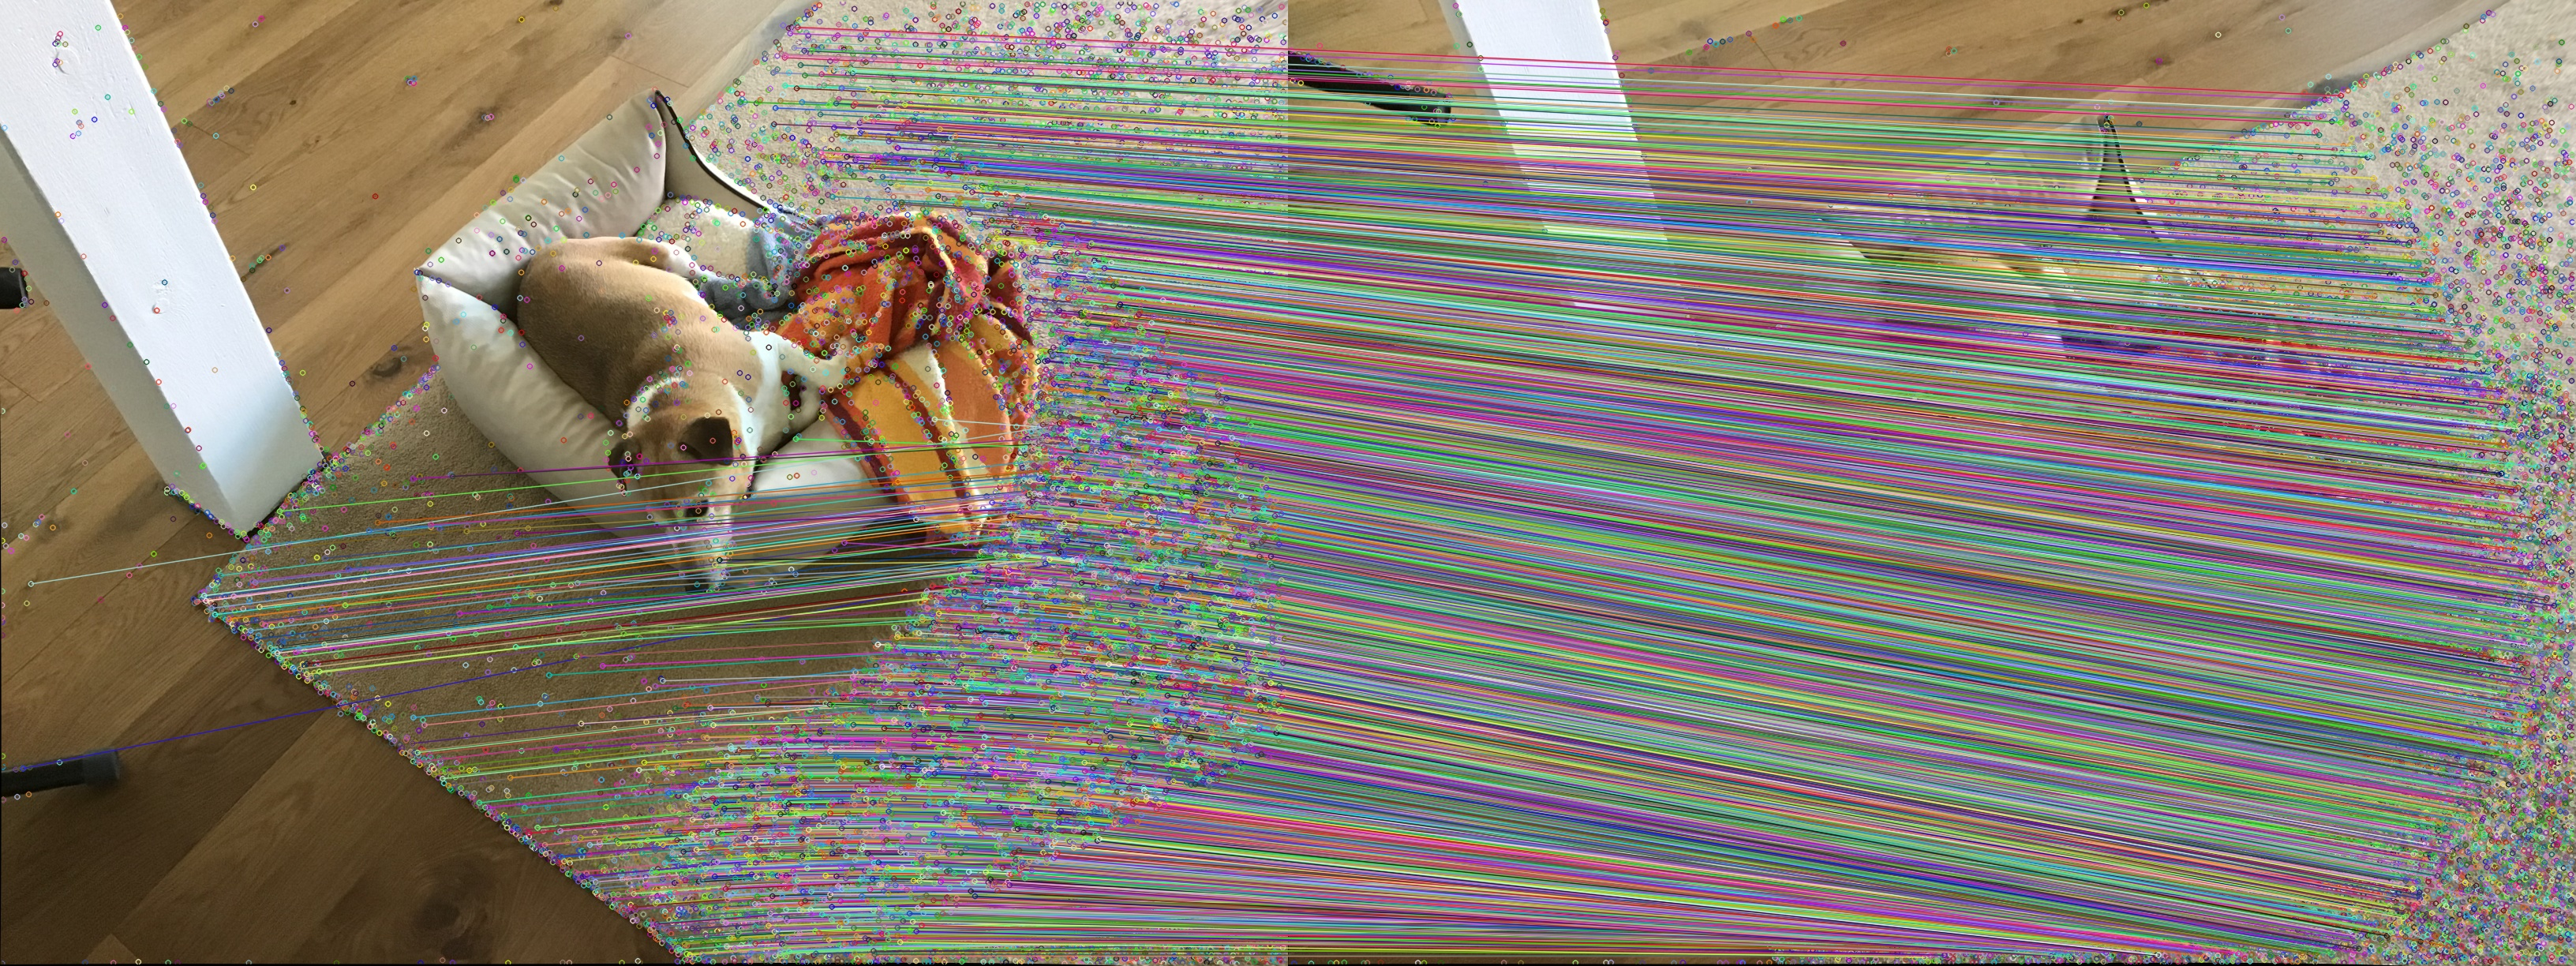
\includegraphics[width=\textwidth]{src/img/dog_first_pair_with_matches.jpg}
    \caption{Das erste der neun 8 Bildpaare, das die Keypoints und ihre Matches zeigt.}
    \label{fig:dog-first-pair-with-matches}
\end{figure}

\begin{figure}
    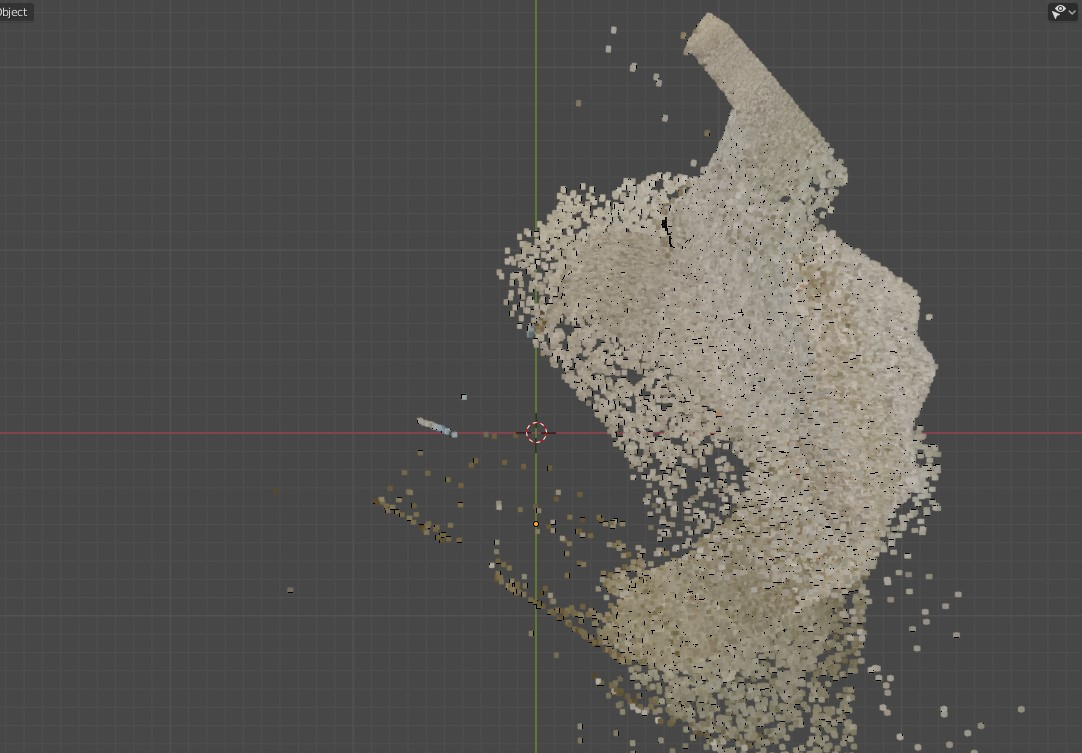
\includegraphics[width=\textwidth]{src/img/dog_model.jpg}
    \caption{Die rekonstruierten Punkte aus den Hundebildern. Das Bild zeigt das Modell ungefähr aus der Position der ersten Kamera.}
    \label{fig:dog-model}
\end{figure}

\begin{figure}
    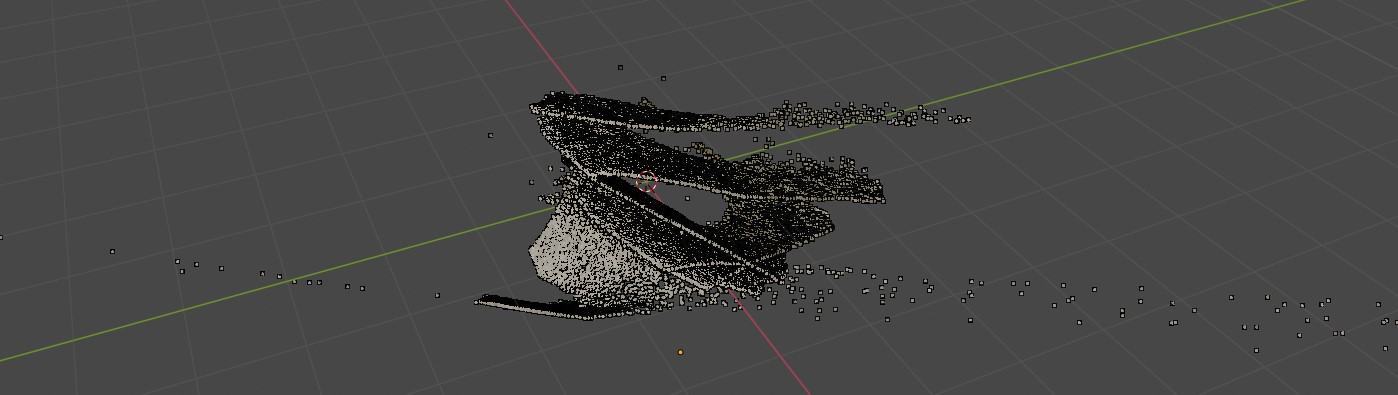
\includegraphics[width=\textwidth]{src/img/dog_model_2.jpg}
    \caption{Die rekonstruierten Punkte aus den Hundebildern. Das Bild zeigt das Modell von der Seite.}
    \label{fig:dog-model-2}
\end{figure}

\section{Fall 4: Box}
\label{sec:testcase-box}\ohead{Sebastian Schmitt}
Im vierten Testfall wird versucht eine Box anhand von fünf Bildern zu rekonstruieren.
Diese ist in \autoref{fig:box-image} zu sehen.

Die \autoref{tab:box-results} zeigt die Ergebnisse der Rekonstruktion.
Es fällt auf, dass nur vergleichsweise sehr wenige Matches gefunden werden.
Betracht man jedoch in \autoref{fig:box-first-pair-with-matches} wo Keypoints und Matches liegen, erkennt man, dass die meisten Matches durchaus direkt an der Box bzw. an dem Kissen auf der Box gefunden wurden.
Besonders das Kissen und die Vorderseite der Box kann man in \autoref{fig:box-model} gut erkennen.
Diese guten Matches kommen zustande, da es in den Bildern klare Flächen mit identifizierbaren Kanten gibt.
Dass auf der Seite der Box keine Matches gefunden wurden, ist dadurch zu erklären, dass jeweils nur ein Bild existiert auf welchem eine Boxseite zu erkennen ist.
Betrachtet man \autoref{fig:box-model-2}, so erkennt man etwas oberhalb deutlich weitere Punkte zu Kissen bzw. Boxdeckel, welche eigentlich tiefer liegen müssten.
Dies lässt ähnlich wie in \autoref{sec:textcase-chair} eine ungenaue Skalierung des Translationsvektors vermuten.

\begin{figure}
    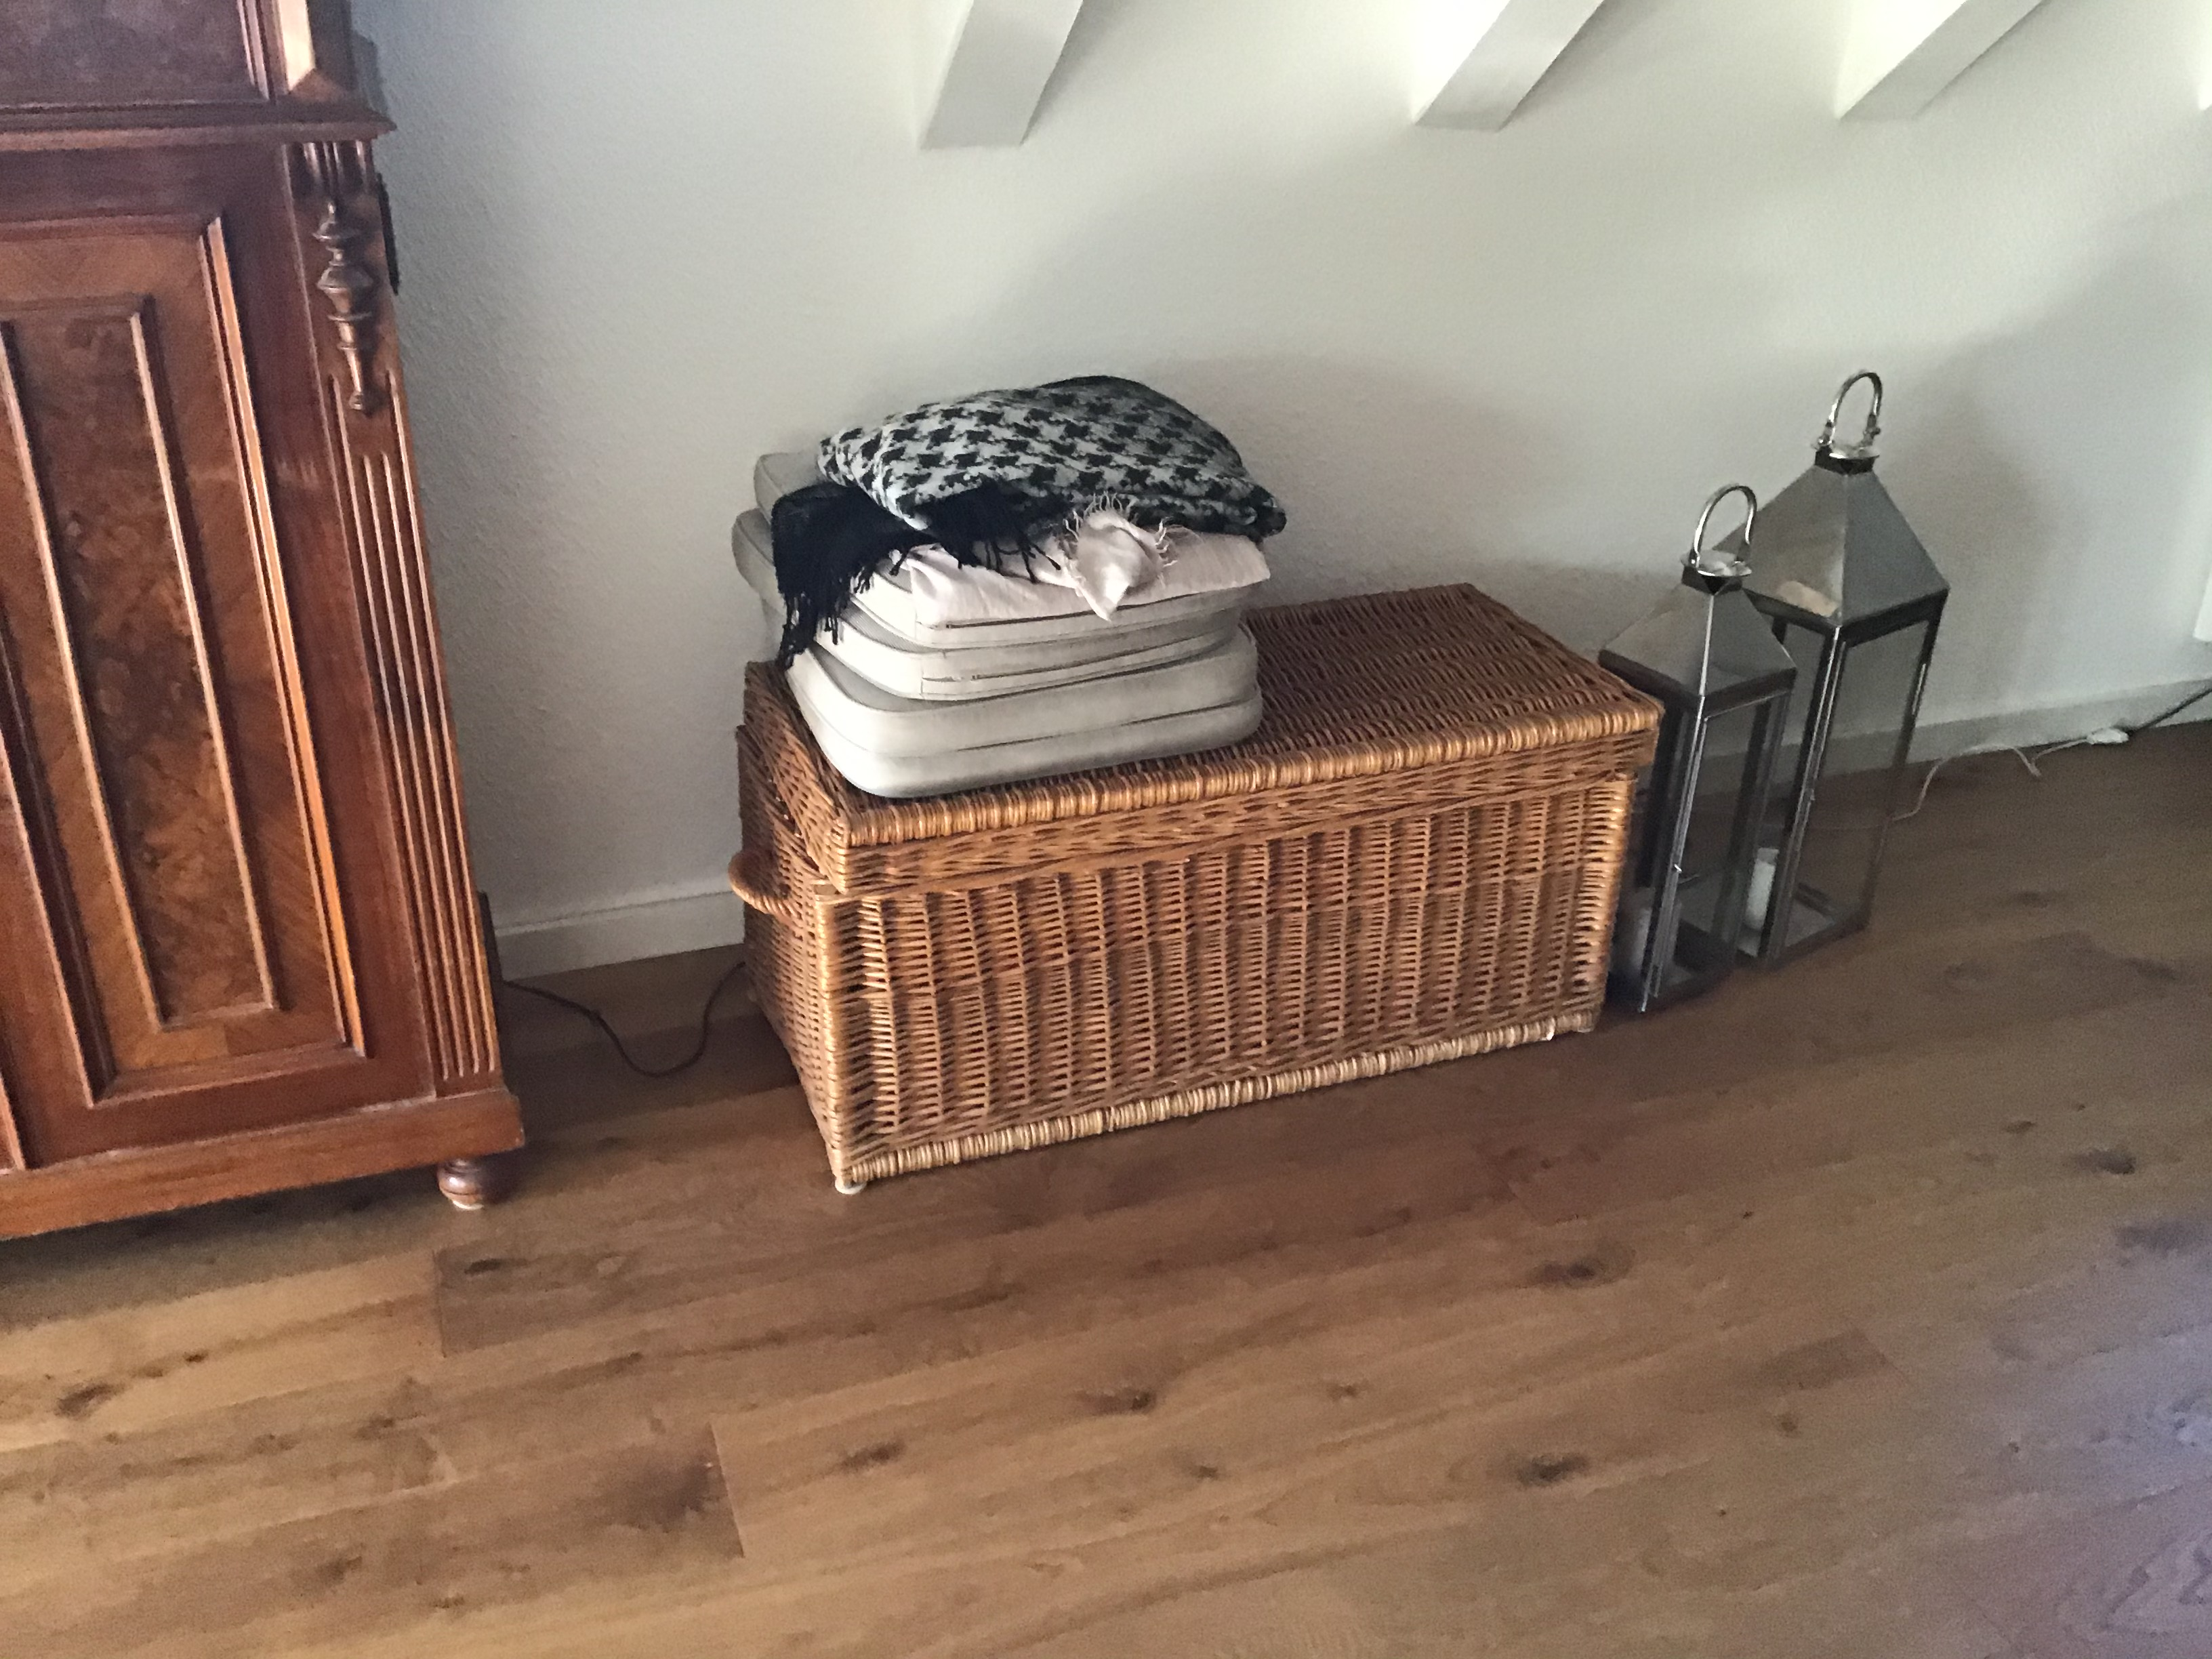
\includegraphics[width=\textwidth]{src/img/box.jpg}
    \caption{Die Box welche rekonstruiert wird}
    \label{fig:box-image}
\end{figure}

\begin{table}
    \begin{tabularx}{\textwidth}{XXXXX}
        \toprule
        Bildpaar &  Anzahl der Matches & Anzahl der Weltpunkte & Anzahl der überlappenden Weltpunkte & angewandte Skalierung \\ 
        \midrule
        1 & 267 & 215 & -  & - \\
        2 & 914 & 215 & 81 & 0,667182 \\
        3 & 433 & 359 & 117 & 1,34628 \\
        4 & 1.170 & 1.154 & 131 & 0,542451 \\
        \midrule
        Summe & 2.786 & 2.542 & 329 & - \\
        \bottomrule
    \end{tabularx}
    \caption{Ergebnis der Rekonstruktion der neun Hundebilder}
    \label{tab:box-results}
\end{table}

\begin{figure}
    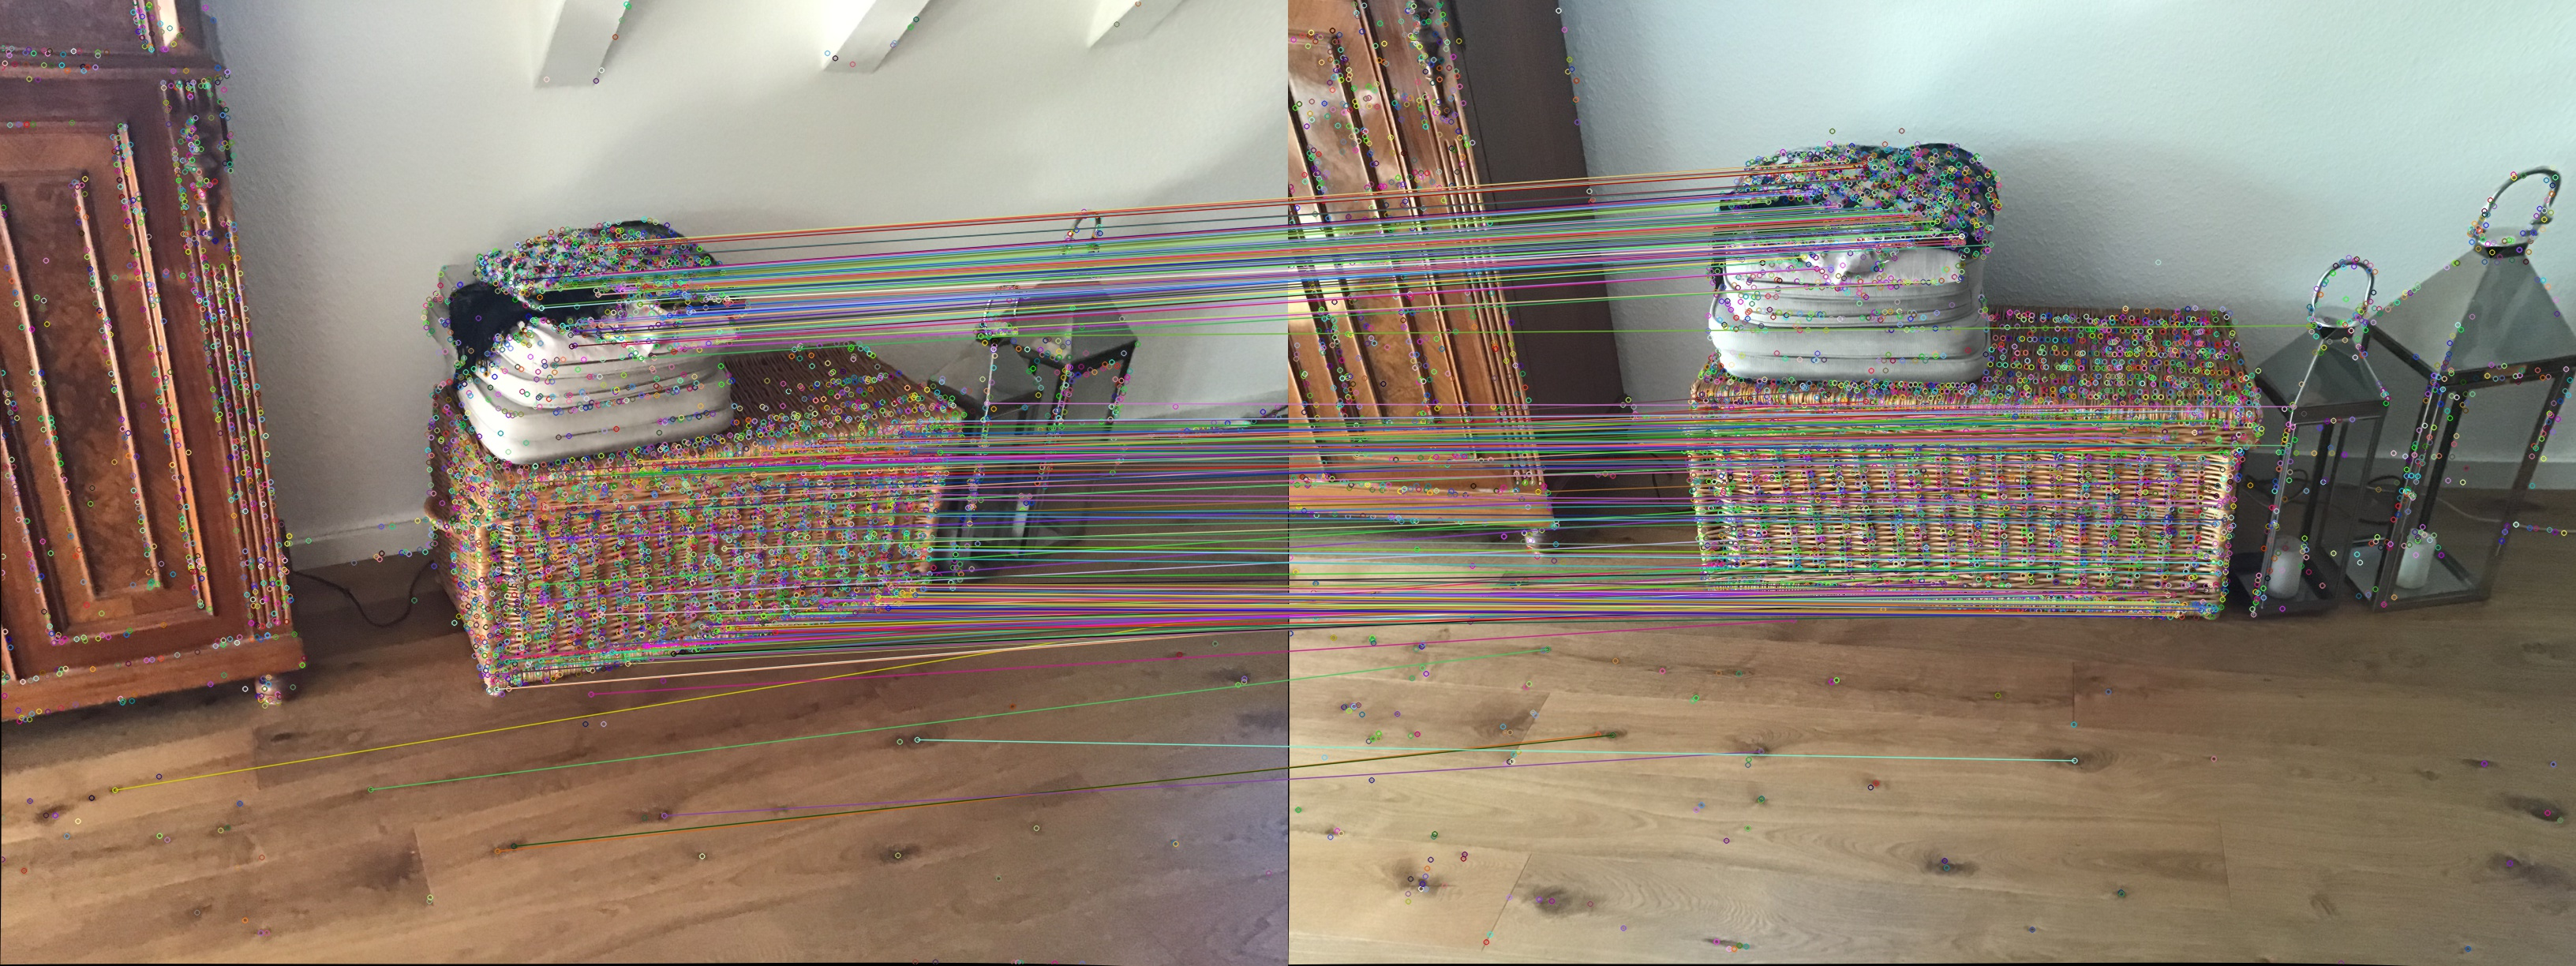
\includegraphics[width=\textwidth]{src/img/box_first_pair_with_matches.jpg}
    \caption{Das erste Bildpaar, mit Matches und Keypoints}
    \label{fig:box-first-pair-with-matches}
\end{figure}

\begin{figure}
    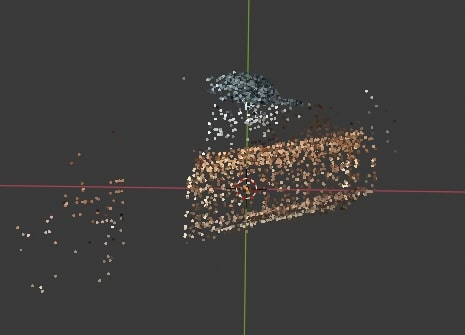
\includegraphics[width=\textwidth]{src/img/box_model.jpg}
    \caption{Die rekonstruierten Punkte aus den Bildern der Box. Das Bild zeigt das Modell ungefähr aus der Position der ersten Kamera.}
    \label{fig:box-model}
\end{figure}

\begin{figure}
    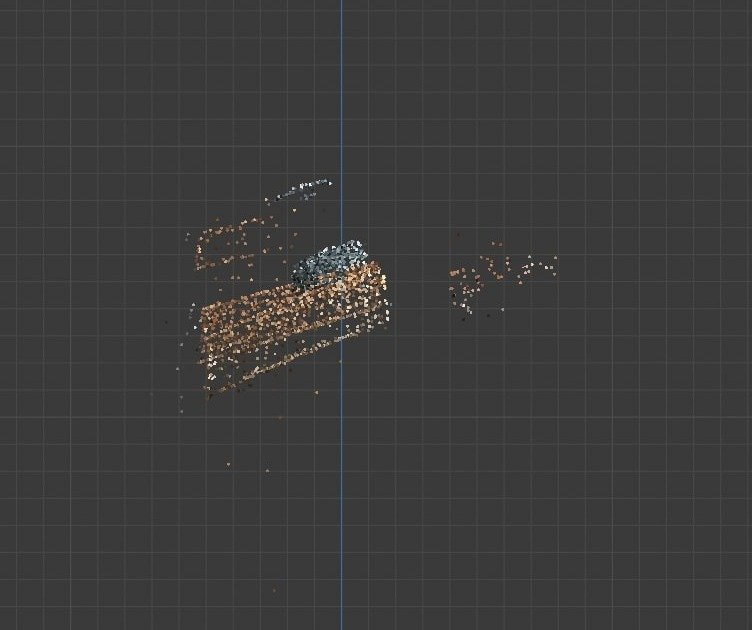
\includegraphics[width=\textwidth]{src/img/box_model_2.jpg}
    \caption{Die rekonstruierten Punkte aus den Bildern der Box. Das Bild zeigt das Modell von der Seite.}
    \label{fig:box-model-2}
\end{figure}
% !TeX root = ../main.tex

\chapter{Fazit}

Lorem ipsum dolor sit amet, consectetur adipiscing elit.
Proin ornare augue eu diam aliquam blandit.
Integer neque metus, semper et urna nec, congue dignissim risus.
Maecenas efficitur tempor malesuada.
Vestibulum mollis sapien a massa porttitor tincidunt.
Duis non iaculis est.
Vestibulum ullamcorper ornare metus, sed pretium nibh facilisis et.
Duis a pellentesque felis.
Suspendisse congue dui metus.
Ut efficitur sodales sollicitudin.
Duis massa nisi, sodales ut felis et, laoreet congue ex.
Donec non lacinia ante.
Nullam sed diam ligula.
Suspendisse sed faucibus libero, non tempor ex. 

\chapter{Ausblick}

\addcontentsline{toc}{chapter}{\protect\numberline{}Literatur}
\printbibliography

% !TeX root = ../main.tex

\addchap{Glossar}

\begin{table}[ht]
    \begin{tabularx}{\textwidth}{l X}
        \toprule
        Begriff & Erläuterung \\
        \midrule
        \bottomrule
    \end{tabularx}
\end{table}


\end{document}
